%\begin{savequote}[8cm]
%  ``Confession: I played golf. Confession: I hired a cleaning lady. Confession: I am owner of the Turbo nose-hair trimmer with optional ear-hair accessory.''
%  \qauthor{Dan Zevin}
%\end{savequote}
%\makeatletter
\chapter{Basics}
\label{Basics}


\section{Notational Conventions}
\label{Basics:Notation}

Every point \nomenclature{$\R$}{The real numbers} $\V{x} \in \R^3 \setminus \set{\V{0}}$ given in Cartesian coordinates by the vector 
$\paren{x_1,x_2,x_3}^{\transp}$ can be uniquely described in spherical coordinates by a vector
$\paren{r,\vtheta,\vphi}^{\transp}$ with $r \in \Rp$, $\vtheta \in \interv{[}{0}{\pi}{]}$ and 
$\vphi \in \interv{[}{0}{2\pi}{)}$.
We have
\begin{eqnarray*}
  \paren{x_1,x_2,x_3}^{\transp} & = & \paren{r \sin \vtheta \cos \vphi, r \sin \vtheta \sin \vphi, r \cos \vtheta}^{\transp}\\
  r & = & \sqrt{x_1^2+x_2^2+x_3^2} = \norm{\V{x}}_2.
\end{eqnarray*} 
We denote by $\twosphere$ the unit sphere embedded into $\R^3$, i.e. 
\[\twosphere := \pset{\V{x} \in \R^{3}}{|}{\norm{\V{x}}_2=1}\] 
and identify $\V{\xi} \in \twosphere$ with the vector $\paren{\vtheta,\vphi}^{\transp}$. The 
spherical coordinate system is illustrated in Figure \ref{sphere}.

Now let $\V{\xi} := \paren{\vtheta,\vphi}^{\transp}$, $\V{\eta} := \paren{\vtheta',\vphi'}^{\transp} \in
\twosphere$ and $\alpha$ be the angle spanned by the origin, $\V{\xi}$ and $\V{\eta}$.
Then the standard inner product
$\V{\xi} \cdot \V{\eta} = \cos \alpha$ is given by
\begin{equation}
  \nonumber
  \cos \alpha = \cos\vtheta\cos\vtheta' +
  \sin\vtheta\sin\vtheta'\fun{\cos}{\vphi-\vphi'}.
\end{equation}

The space of \emph{homogeneous polynomials} of degree $k \in \NZ$ in $\R^3$ is denoted by
$\fun{\text{Hom}_k}{\R^3}$, comprising all polynomials $Q_k \in \Pol_{k}\paren{\R^3}$ fulfilling 
$\fun{Q_k}{\alpha\:\V{x}} = \alpha^k \fun{Q_k}{\V{x}}$ for arbitrary $\alpha \in \R$ and $\V{x}
\in \R^3$. The proper subspace of \emph{harmonic homogeneous polynomials} of
degree $k$ is defined by
\begin{equation}
  \nonumber
  \fun{\text{Harm}_k}{\R^3} := \pset{Q_k \in \fun{\text{Hom}_k}{\R^3}}{|}{\Delta_{\V{x}} Q \equiv 0},
\end{equation}
where $\Delta_{\V{x}}$ is the Laplacian
\begin{equation}
  \nonumber
  \Delta_{\V{x}} = \frac{\partial^2}{\partial x_1^2} + \frac{\partial^2}{\partial x_2^2} +
  \frac{\partial^2}{\partial x_3^2}.
\end{equation}
Furthermore, we have
\begin{align}
  \nonumber
  \fun{\dim}{\fun{\text{Hom}_k}{\R^3}} & = \frac{(k+1)(k+2)}{2}, & 
  \fun{\dim}{\fun{\text{Harm}_k}{\R^3}} = 2k+1.
\end{align}
To keep it short, we let $\Pol_{k}\paren{\twosphere} := \left.\Pol_{k}\paren{\R^3}\right|_{\twosphere}$ and 
$\mathcal{H}_k := \left.\fun{\text{Harm}_k}{\R^3}\right|_{\twosphere}$. For 
further information, see for example \cite[Chapter 2.3]{frgesc}.

\begin{figure}[tb]
  \centering
  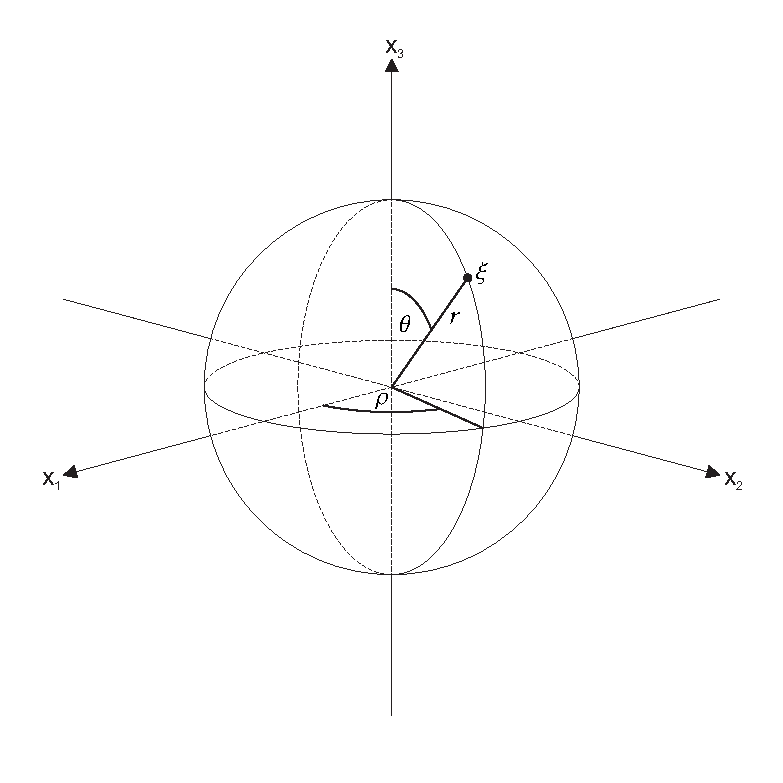
\includegraphics[width=0.87\textwidth]{images/sphere}
  \caption{The spherical coordinate system in $\R^3$. Every point $\V{\xi}$ on a
  sphere with radius $r$ around the origin can be uniquely described by angles 
  $\vtheta$, $\vphi$ and the radius $r$. For $\vtheta = 0$ or
  $\vtheta = \pi$ the point $\V{\xi}$ coincides with the North or the South
  pole, respectively.}
  \label{sphere}
\end{figure}

\section{Legendre Functions}
\label{Basics:LegendreTypeFunctions}
In this section, we briefly introduce \emph{Legendre polynomials}, \emph{associated Legendre functions} 
and \emph{associated Legendre polynomials} and collect basic properties. These functions play 
a major role in Fourier analysis on the sphere and are key for the algorithms related to Fourier 
expansions, developed in this text.

The Legendre polynomials $P_k : \interv{[}{-1}{1}{]} \rightarrow \R$, $k \in \N_{0}$ 
as classical orthogonal polynomials are given by their corresponding 
\emph{Rodrigues formula}
\begin{equation}
  \nonumber
  \fun{P_k}{x} := \frac{1}{2^k k!} \frac{\dx^k}{\dx x^k} \paren{x^2-1}^k.
\end{equation}
One verifies $\fun{P_{k}}{\pm1} = \paren{\pm1}^{k}$, $\left|\fun{P_{k}}{\cos\vartheta}\right|
\le \sqrt{\frac{2}{\pi k \sin\vartheta}}$ for $\vartheta \in (0,\pi)$, $k \ge 1$, 
and $\max_{x \in \interv{[}{-1}{1}{]}} \abs{\fun{P_{k}}{x}} = 1$ (see \cite[pp. 47]{niuv}).
Two recurrence relations are given by
\begin{equation}
  \label{three1}
  \paren{k+1}\fun{P_{k+1}}{x} = \paren{2k+1}x\fun{P_{k}}{x} - k\fun{P_{k-1}}{x}
\end{equation}
and
\begin{equation}
  \label{three2}
  \paren{2k+1} \fun{P_{k}}{x} = \fun{P_{k+1}'}{x} - \fun{P_{k-1}'}{x}.
\end{equation}
Furthermore, we define the associated Legendre functions $P_k^n : \interv{[}{-1}{1}{]} \rightarrow \R$ by
\begin{equation}
  \nonumber
  \fun{P_k^n}{x} := \sqrt{\frac{\paren{k-n}!}{\paren{k+n}!}}
  \paren{1-x^2}^{n/2} \frac{\dx^n}{\dx x^n} \fun{P_k}{x} \quad \paren{n \in \NZ,\ k=n,n+1,\ldots}.
\end{equation}
For fixed $n$, the set $\set{P_{k}^n}_{k=n,n+1,\ldots}$ forms a complete set of orthogonal functions 
for $\Ln{2}{[-1,1]}$ with
\[ 
  \scalarproduct{P_{k}^n}{P_{l}^n}_{\Ln{2}{[-1,1]}} := \int_{-1}^{1} \fun{P_{k}^n}{x} 
  \fun{P_{l}^n}{x} \dx x = \frac{2}{2k+1} \delta_{k,l} \quad \paren{0 \le n \le k,l}.
\]
The associated Legendre functions obey the three-term recurrence relation
\begin{equation}
  \label{Basics:AssociatedLegendreDefinition}
  \begin{split}
    \fun{P_{n-1}^n}{x} & := 0,\qquad \fun{P_{n}^n}{x} := \frac{\sqrt{(2n)!}}{2^n n!} \paren{1-x^2}^{n/2},\\
    \fun{P_{k+1}^n}{x} & = v_{k}^n x \fun{P_{k}^n}{x} + w_{k}^n \fun{P_{k-1}^n}{x} \quad (k = n,n+1,\ldots),
  \end{split}
\end{equation}
where
\begin{equation} 
  \label{Basics:AssociatedLegendreRecurrenceCoefficients}
v_{k}^n := \frac{2k+1}{((k-n+1)(k+n+1))^{1/2}}\; ,\qquad w_{k}^n := - \frac{((k-n)(k+n))^{1/2}}{((k-n+1)(k+n+1))^{1/2}}.
\end{equation}
A simple but at the same time very powerful idea is to define the associated Legendre functions $P_k^n$ also for 
$k < n$ by means of the modified three-term recurrence
\begin{equation} 
  \label{Basics:AssociatedLegendreDefinitionExtended}
  \fun{P_{k+1}^n}{x} = \paren{\alpha_{k}^n x + \beta_{k}^n} \fun{P_{k}^n}{x} + \gamma_{k}^n \fun{P_{k-1}^n}{x}\quad\paren{k \in \NZ}
\end{equation}
with
\begin{equation}
  \label{Basics:AssociatedLegendreRecurrenceCoefficientsExtended}
  \begin{split}
	  \alpha_{k}^n & := \left\{
	    \begin{array}{ll}
	      (-1)^{k+1} & \text{for}\ k < n,\\
	      v_{k}^n    & \text{otherwise},
	    \end{array}\right.\\
	  \beta_{k}^n & := \left\{
	    \begin{array}{lll}
	      1 & \text{for}\ k < n,\\
	      0 & \text{otherwise},
	    \end{array}\right.\\
	  \gamma_{k}^n & := \left\{
	    \begin{array}{lll}
	      0       & \text{for}\ k \leq n,\\
	      w_{k}^n & \text{otherwise.}
	    \end{array}\right.
	\end{split}  
\end{equation}
For even $n$, we let
\[ 
  \fun{P_{-1}^n}{x} := 0,\ \fun{P_{0}^n}{x} := \frac{\sqrt{(2n)!}}{2^n n!},
\]
and for odd $n$, we start with
\[ \fun{P_{0}^n}{x} := \fun{P_{1}^n}{x} := \frac{\sqrt{(2n)!}}{2^n n!} \paren{1-x^2}^{1/2}.\]
For $k \ge n$, this definition coincides with \eqref{Basics:AssociatedLegendreDefinition}. 
As a matter of fact, $P_{k}^n$ is a polynomial of degree $k$ for even $n$ while 
$\paren{1-x^2}^{-1/2}P_{k}^n$ is a polynomial of degree $k-1$ for odd $n$.

Based on the recurrence coefficients from \eqref{Basics:AssociatedLegendreRecurrenceCoefficientsExtended} 
and introducing a shift parameter $c \in \NZ$, we 
define the associated Legendre polynomials $\fun{P_{k}^n}{\cdot,c}$ by
\begin{equation}
  \label{Basics:AssociatedLegendrePolynomials}
  \begin{split}
    & \fun{P_{-1}^n}{x,c} := 0,\ \fun{P_{0}^n}{x,c} := 1,\\
    & \fun{P_{k+1}^n}{x,c} = \paren{\alpha_{k+c}^n x + \beta_{k+c}^n} \fun{P_{k}^n}{x,c} + \gamma_{k+c}^n \fun{P_{k-1}^n}{x,c}.
  \end{split}
\end{equation}
We have the following Lemma:
\begin{lemma}
  \label{Basics:AssociatedLegendreRecurrence}
  Let $c \ge 1$, $k \ge 0$ and the functions $P_{k}^n$ and $\fun{P_{k}^n}{\cdot,c}$ be given as in 
  \eqref{Basics:AssociatedLegendreDefinitionExtended}, 
  \eqref{Basics:AssociatedLegendreRecurrenceCoefficientsExtended}, and 
  \eqref{Basics:AssociatedLegendrePolynomials}. 
  Then we have
  \[ 
    \fun{P_{c+k}^n}{x} = \fun{P_{k}^n}{x,c} \fun{P_{c}^n}{x} + \gamma_{c}^n \fun{P_{k-1}^n}{x,c+1} \fun{P_{c-1}^n}{x}.
  \]
\end{lemma}
\begin{proof}
  The proof is by induction over $k$. So let $c \ge 1$ be arbitrary. For $k = 0,1$ we have
  \begin{align}
    \nonumber
    \fun{P_{c+0}^n}{x} 
%    & = 1 \; \fun{P_{c}^n}{x} + \gamma_{c}^n \; 0 \; \fun{P_{c-1}^n}{x},\\
%    \nonumber
    & = \fun{P_{0}}{x,c}\fun{P_{c}^n}{x} + \gamma_{c}^n \fun{P_{-1}}{x,c} \fun{P_{c-1}^n}{x},\\
    \nonumber
    \fun{P_{c+1}^n}{x} 
    & = \paren{\alpha_{c}^n x + \beta_{c}^n} \fun{P_{c}^n}{x} + \gamma_{c}^n \fun{P_{c-1}^n}{x}\\
    \nonumber
    & = \fun{P_{1}}{x,c}\fun{P_{c}^n}{x} + \gamma_{c}^n \fun{P_{0}}{x,c} \fun{P_{c-1}^n}{x}.
  \end{align}
  Let now the assertion be true for $k$ and $k-1$, where $k \ge 1$ is fixed. We verify
  \begin{equation}
    \nonumber
    \begin{split}
      \fun{P_{c+k+1}^n}{x}& 
       = \paren{\alpha_{c+k}^n x + \beta_{c+k}^n} \fun{P_{c+k}^n}{x} + \gamma_{c+k}^n \fun{P_{c+k-1}^n}{x}\\
      & = \paren{\alpha_{c+k}^n x + \beta_{c+k}^n} \paren{\fun{P_{k}^n}{x,c} \fun{P_{c}^n}{x} + 
      \gamma_{c}^n \fun{P_{k-1}^n}{x,c+1} \fun{P_{c-1}^n}{x}}\\
      & \quad + \gamma_{c+k}^n \paren{\fun{P_{k-1}^n}{x,c} \fun{P_{c}^n}{x} + 
      \gamma_{c}^n \fun{P_{k-2}^n}{x,c+1} \fun{P_{c-1}^n}{x}}\\
      & = \paren{\paren{\alpha_{c+k}^n x + \beta_{c+k}^n}\fun{P_{k}^n}{x,c} + \gamma_{c+k}^n\fun{P_{k-1}^n}{x,c}} \fun{P_{c}^n}{x}\\ 
      & \quad + \gamma_{c}^n\paren{\paren{\alpha_{c+k}^n x + \beta_{c+k}^n}\fun{P_{k-1}^n}{x,c+1} + \gamma_{c+k}^n\fun{P_{k-2}^n}{x,c+1}}\fun{P_{c-1}^n}{x}\\ 
      & = \fun{P_{k+1}^n}{x,c} \fun{P_{c}^n}{x} + \gamma_{c}^n \fun{P_{k}^n}{x,c+1} \fun{P_{c-1}^n}{x}
    \end{split}  
  \end{equation}
\end{proof}

\section{Spherical Harmonics}
\label{Basics:SphericalHarmonics}

\emph{Spherical harmonics} on the sphere $\twosphere$ arise the same way as complex exponentials 
$\e^{\im n x}$, $n \in \Z$, on the unit circle $\mathbb{S}^1$. In cartesian coordinates, they are 
homogeneous harmonic polynomials in $\R^3$, but restricted to $\twosphere$. For a brief 
comprehensive introduction, we refer to \cite{Mo99}. A more general and abstract treatment is
found in \cite{frgesc}.

In $\R^2$, a homogeneous harmonic polynomial $p_{n}$ of degree $n \in \NZ$, restricted to the unit 
circle $\mathbb{S}^1$ must fulfill 
\[
  n^2 \fun{q_{n}}{\vphi} + \fun{q_{n}''}{\vphi} = 0
\]
in polar coordinates $\vphi \in [-\pi,\pi)$. Equivalently, $q_{n}$ is 
an eigenfunction of the \emph{circular Laplacian} $\Delta_{\vphi} = \frac{\partial^2}{\partial \vphi^2}$ 
corresponding to the eigenvalue $n^2$.
Following these lines, a homogeneous harmonic polynomial $q_{k} \in \fun{\Pi}{\R^3}$ in spherical coordinates, 
restricted to the unit sphere $\twosphere$,
is an eigenfunction of the \emph{spherical Laplacian} or \emph{Laplace-Beltrami operator} 
\[
  \Delta_{\paren{\vtheta,\vphi}} = \frac{1}{\sin^2 \vtheta} 
  \frac{\partial^2}{\partial \vphi^2} + \frac{1}{ \sin \vtheta}�
   \frac{\partial}{\partial \vtheta} \paren{\sin \vtheta \: \frac{\partial}{\partial \vtheta}}.
\]
with eigenvalue $k(k-1)$ and obeys
\begin{equation}
  \label{Basics:LaplaceBeltrami}
  \Delta_{\paren{\vtheta,\vphi}} \fun{q_{k}}{\vtheta,\vphi} = -k(k-1) \fun{q_{k}}{\vtheta,\vphi}.
\end{equation}
Using an ansatz based on separation of variables (see \cite{co2}), one obtains the linear independent solutions
\begin{equation}
  \label{Basics:SphericalHarmonicsDefinition}
  \begin{split}
    & Y_{k}^n: \twosphere \rightarrow \C \quad \paren{k \in \NZ,\; n = -k,\ldots,k},\\
    & \fun{Y_{k}^n}{\vtheta,\vphi} := \sqrt{\frac{2k+1}{4\pi}} 
    \fun{P_{k}^{\abs{n}}}{\cos \vtheta} \e^{\im n \vphi}.
  \end{split}
\end{equation}
The index $k$ is called the \emph{degree} and $n$ is denoted the \emph{order} of $Y_{k}^n$. 
Figure \ref{Basics:Figure:SphericalHarmonics} illustrates several functions $Y_{k}^{n}$.
Due to the separability with respect to $\vtheta$ and $\vphi$, one proves easily the 
orthogonality property
\begin{equation}
  \label{Basics:orthogonality}
  \scalarproduct{Y_{k}^n}{Y_{l}^m}_{\Ln{2}{\twosphere}} = \delta_{k,l} \delta_{n,m}
\end{equation}
with respect to the $\Ln{2}{\twosphere}$-inner product 
\begin{equation}
  \nonumber
  \scalarproduct{Y_{k}^n}{Y_{l}^m}_{\Ln{2}{\twosphere}} = \int_{\twosphere}
  \fun{Y_{k}^n}{\V{\xi}} \overline{\fun{Y_{l}^m}{\V{\xi}}} \: \dx \V{\xi} := 
  \int_{0}^{2\pi} \int_{0}^{\pi} \fun{Y_{k}^n}{\vtheta,\vphi} 
  \overline{\fun{Y_{l}^m}{\vtheta,\vphi}} \sin \vtheta \; 
  \dx \vtheta \; \dx \vphi.
\end{equation}
An important result states $Y_{k}^n \in \mathcal{H}_k$ and therefore, the set
\begin{equation}
  \nonumber
  \pset{Y_{k}^n}{|}{n = -k,\ldots,k}
\end{equation}
forms an orthonormal basis of $ \mathcal{H}_k$, since $\dim \mathcal{H}_k =
2k+1$. Moreover, due to \eqref{Basics:orthogonality}, the spaces $\mathcal{H}_k$ are orthogonal
to each other and
\begin{equation}
  \label{Basics:FourierBasis}
  \pset{Y_{k}^n}{|}{k = 0,\ldots,M;\ n = -k,\ldots,k} \quad \paren{M \in \NZ}
\end{equation}
provides an orthonormal basis for the space $\bigoplus_{k=0}^{M}\mathcal{H}_k$, called
the space of \emph{spherical harmonics} of degree $M$.

At first glance, the restriction to homogeneous and harmonic polynomials
might exclude various functions from $\fun{\Pol_M}{\twosphere}$. But as a 
matter of fact, these spaces are identical (see \cite[Corollary 2.2.5]{frgesc}), i.e. 
\begin{equation}
  \nonumber
    \fun{\Pol_M}{\twosphere} = \bigoplus_{k=0}^{M}\mathcal{H}_k \quad \paren{M \in \NZ}.
\end{equation}
Since polynomials are dense in $\Ln{2}{\twosphere}$, we have also obtained an orthonormal 
basis for $\Ln{2}{\twosphere}$ and we call \eqref{Basics:FourierBasis} the 
\emph{Fourier Basis} for $\Ln{2}{\twosphere}$.
A function $f \in \Ln{2}{\twosphere}$ can be developed into a series
\[
  f = \sum_{k=0}^{\infty} \sum_{n=-k}^{k} a_{k}^n Y_{k}^n,
\]
where the coefficients $a_{k}^n = \fun{f^{\wedge}}{k,n} = \scalarproduct{f}{Y_{k}^{n}}_{\Ln{2}{\twosphere}}$
are the \emph{spherical Fourier coefficients}.
\begin{remark}
  There exist several different denotations for the functions $Y_{k}^n$. ...
\end{remark}
%one obtains from Laplace's differential equation $\Delta_{\V{x}} f \equiv 0$ in $\R^3$ in spherical coordinates
%i.e. as restrictions of homogeneous harmonic polynomials  and form 
%a complete orthogonal system for $\Ln{2}{\twosphere}$.
%Speaking of Fourier analysis with respect to the sphere, one refers to a set of certain 
%functions $Y_{k}^n$ for $k \in \NZ$, $|n| \le k$ as the Fourier basis on $\twosphere$. 

\begin{figure}[hp]
  \centering
   \subfigure[$\Re \: Y_{0}^{0}$]
     {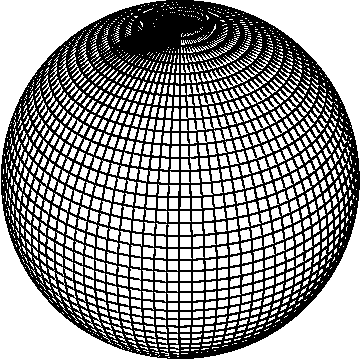
\includegraphics[width=0.33\textwidth]{images/sh_r_0_0}}\hfill
   \subfigure[$\Re \: Y_{4}^{2}$]
     {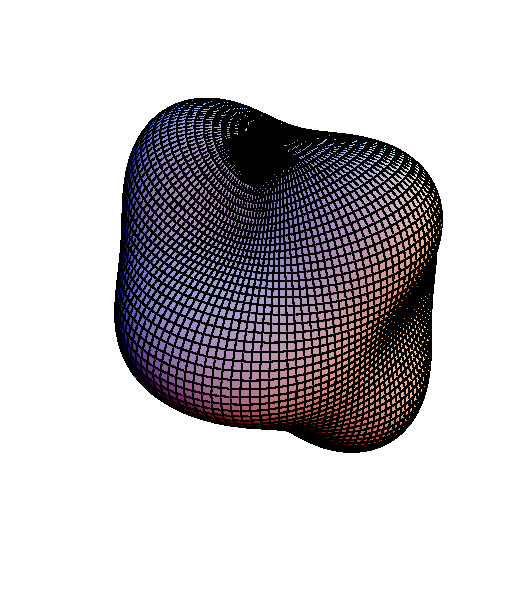
\includegraphics[width=0.33\textwidth]{images/sh_r_4_2}}\\
   \subfigure[$\Re \: Y_{9}^{5}$]
     {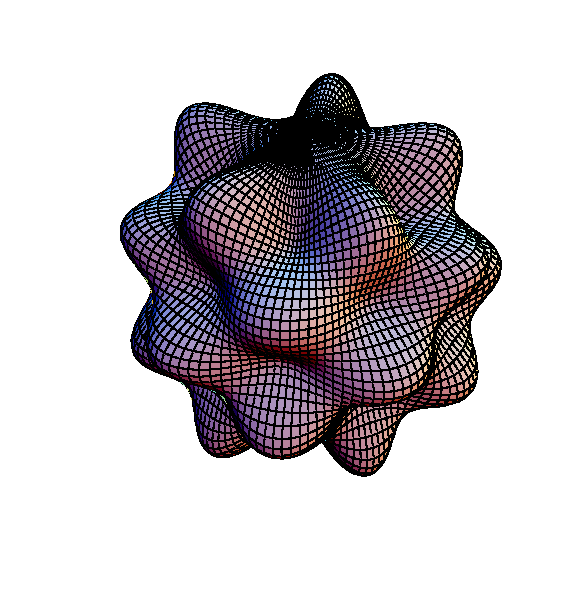
\includegraphics[width=0.33\textwidth]{images/sh_r_9_5}}\hfill
   \subfigure[$\Re \: Y_{13}^{1}$]
     {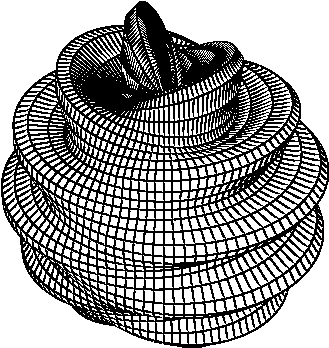
\includegraphics[width=0.33\textwidth]{images/sh_r_13_1}}\\
   \subfigure[$\Re \: Y_{13}^{6}$]
     {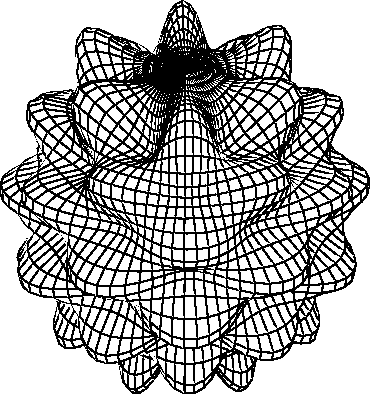
\includegraphics[width=0.33\textwidth]{images/sh_r_13_6}}\hfill
   \subfigure[$\Re \: Y_{13}^{13}$]
     {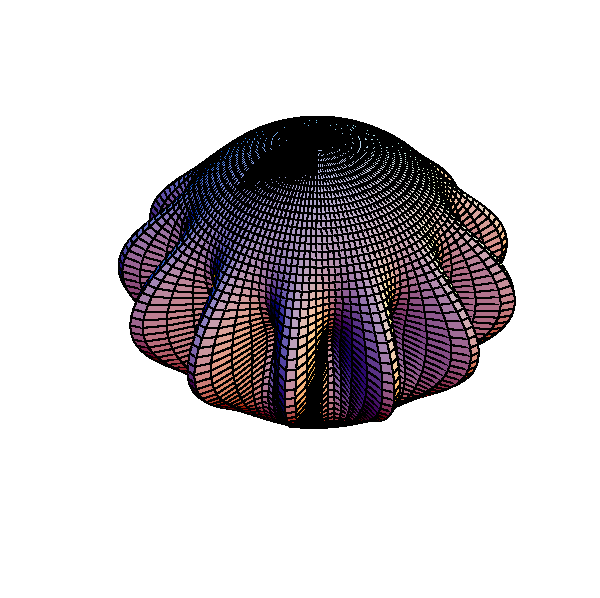
\includegraphics[width=0.33\textwidth]{images/sh_r_13_13}}\\
  \caption{The real part of $Y_{k}^{n}$ for different combinations $\paren{k,n}$.}
  \label{Basics:Figure:SphericalHarmonics}
\end{figure}

We finally mention the fundamental and well known \emph{Addition theorem} for spherical harmonics 
that relates any set of functions $\set{H_k^n}_{n=-k}^k$ forming an orthonormal basis of $\mathcal{H}_k$ 
to the Legendre polynomials $P_{k}$.

\begin{proposition}[Addition Theorem]
  \label{Basics:AdditionTheorem}
  For every $\Ln{2}{\twosphere}$-orthonormal basis\\ 
  $\set{H_{k}^n}_{n=-k}^{k}$ of $\mathcal{H}_k$, $k \in \NZ$, we have
  \begin{equation}
    \nonumber
    \sum_{n=-k}^{k} \fun{H_{k}^n}{\V{\xi}} \overline{\fun{H_{k}^n}{\V{\eta}}} =
    \frac{2k+1}{4\pi}\fun{P_k}{\V{\xi} \cdot \V{\eta}}.
  \end{equation}
\end{proposition}

See \cite[p. 37]{frgesc} or \cite[pp. 172, Theorem 5]{co} for a proof. In particular, the theorem 
holds for the basis functions $Y_{k}^n$.

\section{Spherical Radial Basis Functions}
\label{Basics:SphericalKernels}

\emph{Spherical radial basis functions} are the spherical counterpart 
of \emph{radial basis functions} in Euclidean spaces (see for example 
\cite{buhmann} or \cite{wendland}). Other denotations are \emph{spherical radial kernels} or
\emph{zonal functions}.
Generally, one starts with a function $K$ from $\Ln{2}{\interv{[}{-1}{1}{]}}$
and defines for fixed $\V{\eta} \in \twosphere$ the $\V{\eta}$-zonal function 
\[
  \fun{K}{\V{\eta} \: \cdot}: \twosphere \rightarrow \C,\ \V{\xi} \mapsto \fun{K}{\V{\eta} \cdot \V{\xi}} \quad \paren{\V{\xi} \in \twosphere}.
\]
The fact that the geodesic distance $d$ for two points $\V{\eta}$, $\V{\xi} \in \twosphere$ is $\fun{d}{\V{\eta},\V{\xi}} = 
\sqrt{2-2\V{\eta}\cdot\V{\xi}}$ justifies the name \emph{spherical radial basis function}. 
By means of the \emph{Funk-Hecke formula} (see \cite[pp. 60]{frgesc}) we obtain for fixed $k \in \NZ$
\begin{equation}
  \label{Basics:Symbol2}
  \scalarproduct{\fun{K}{\V{\eta} \: \cdot}}{Y_{k}^n}_{\Ln{2}{\twosphere}} = \int_{\twosphere} 
  \fun{K}{\V{\eta} \cdot \V{\xi}} \overline{\fun{Y_{k}^n}{\V{\xi}}} \: \dx \V{\xi} = 
  \fun{K^{\wedge}}{k} \overline{\fun{Y_{k}^n}{\V{\eta}}} \quad \paren{n=-k,\ldots,k},
\end{equation}
where the \emph{Legendre transform} is given by
\begin{equation}
  \label{Basics:Symbol}
  \fun{K^{\wedge}}{k} := 2 \pi \int_{-1}^{1} \fun{K}{x} \fun{P_{k}}{x} \dx x \quad \paren{k \in \NZ}.
\end{equation}
We have therefore 
\begin{equation}
  \label{Basics:Kernel}
  \fun{K}{\V{\eta} \cdot \V{\xi}} = \sum_{k = 0}^{\infty} \sum_{n=-k}^k \fun{K^{\wedge}}{k} 
  \overline{\fun{Y_{k}^n}{\V{\eta}}} \fun{Y_{k}^n}{\V{\xi}} 
\end{equation}
and applying the Addition Theorem from Proposition \ref{Basics:AdditionTheorem}, we obtain 
for $K$ the orthogonal expansion
\begin{equation}
\label{Basics:OrthogonalKernelExpansion}
  \fun{K}{x} = \sum_{k = 0}^{\infty} \frac{2k+1}{4\pi} \fun{K^{\wedge}}{k} \fun{P_k}{x} \quad \paren{x \in \interv{[}{-1}{1}{]}}.
\end{equation}
\begin{remark}
  The Legendre transform $\fun{K^{\wedge}}{k}$ is also called the $symbol$ of $K$ since it corresponds to a
  linear operator $\Lambda: \Ln{2}{\twosphere} \rightarrow \Ln{2}{\twosphere}$ with 
  $\fun{\paren{\Lambda f}^{\wedge}}{k,n} = \fun{K^{\wedge}}{k} \fun{f^{\wedge}}{k,n}$.
\end{remark}
The symbol $\fun{K^{\wedge}}{k}$ has many remarkable properties. The following result allows for the 
construction of so-called \emph{iterated spherical radial basis functions} by multiplying simple the corresponding symbols (see \cite{frsc}).
\begin{lemma}
  Let $P,Q\in \Ln{2}{\interv{[}{-1}{1}{]}}$ and
  \[
  \fun{K}{\V{\eta} \cdot \V{\xi}} := \fun{\left(P * Q\right)}{\V{\eta} \cdot
    \V{\xi}},
  \]
  where
  \begin{equation}
    \label{Basics:Convolution}
    \fun{\left(P * Q\right)}{\V{\eta} \cdot \V{\xi}}:= 
    \int_{\twosphere} \fun{P}{\V{\eta} \cdot \V{\nu}}
    \fun{Q}{\V{\nu} \cdot \V{\xi}} \dx \V{\nu}
  \end{equation}
  is the \emph{spherical convolution} of $Q$ and $P$. Then the symbol 
  $\fun{K^{\wedge}}{k}$ is given by 
  $\fun{K^{\wedge}}{k} = \fun{P^{\wedge}}{k} \fun{Q^{\wedge}}{k}$.
  Furthermore, for compactly supported functions, $\supp\; P = \supp\; Q =
  \interv{[}{h}{1}{]}$, $h \in [0,1]$, we have $\supp\; K =
  \interv{[}{2h^2-1}{1}{]}$.
\end{lemma}
\begin{proof}
  First, we use \eqref{Basics:Symbol2} to get
  \begin{equation}
    \begin{split}
      \scalarproduct{\fun{K}{\V{\eta} \: \cdot}}{Y_{k}^n}_{\Ln{2}{\twosphere}} 
      & = \int_{\twosphere} \fun{K}{\V{\eta} \cdot \V{\xi}} \overline{\fun{Y_{k}^n}{\V{\xi}}} \: \dx \V{\xi}\\
      & = \int_{\twosphere} \int_{\twosphere} \fun{P}{\V{\eta} \cdot \V{\nu}}
          \fun{Q}{\V{\nu} \cdot \V{\xi}} \: \dx \V{\nu} \; \overline{\fun{Y_{k}^n}{\V{\xi}}} \: \dx \V{\xi}\\
      & = \int_{\twosphere} \int_{\twosphere} \fun{Q}{\V{\nu} \cdot \V{\xi}} \overline{\fun{Y_{k}^n}{\V{\xi}}} \:
          \dx \V{\xi} \; \fun{P}{\V{\eta} \cdot \V{\nu}} \: \dx \V{\nu}\\
      & = \int_{\twosphere} \fun{Q^{\wedge}}{k} \fun{P}{\V{\eta} \cdot \V{\nu}} 
          \overline{\fun{Y_{k}^n}{\V{\nu}}} \: \dx \V{\nu}\\
      & = \fun{Q^{\wedge}}{k} \fun{P^{\wedge}}{k} \overline{\fun{Y_{k}^n}{\V{\eta}}}, 
    \end{split}
  \end{equation}  
  which proves $\fun{K^{\wedge}}{k} = \fun{P^{\wedge}}{k} \fun{Q^{\wedge}}{k}$. 
  If $P$ and $Q$ are compactly supported, with $\supp\; P = \supp\; Q =
  \interv{[}{h}{1}{]}$, and $h \in [0,1]$, we note that the support of $P$ and $Q$ 
  are spherical caps $\fun{C_{\V{\eta}}}{h}$ and $\fun{C_{\V{\nu}}}{h}$, respectively, where
   $\fun{C_{\V{\eta}}}{h} := \pset{\V{\xi} \in \twosphere}{|}{\V{\eta} \cdot \V{\xi} \ge h}$. For the 
   integrand in \eqref{Basics:Convolution} not to vanish, we must require $\V{\nu}$ and $\V{\xi}$ to lie in the 
   spherical caps $\fun{C_{\V{\eta}}}{h}$ and $\fun{C_{\V{\nu}}}{h}$. Equivalently, if we denote
   by $\alpha$, $\beta$, $\gamma$ the angles $\fun{\angle}{\V{\eta},\V{\nu}}$, $\fun{\angle}{\V{\nu},\V{\xi}}$, and
   $\fun{\angle}{\V{\eta},\V{\xi}}$, we conclude $\gamma \le \alpha + \beta \le 2 \arccos h$, where we note that
   this estimate is sharp. Since $\fun{\cos}{2 \arccos h} = 2h^2-1$, the support of $K$ is $\supp\; K = \interv{[}{2h^2-1}{1}{]}$.
\end{proof}

The following examples are taken from \cite{frgesc} or \cite{frsc}. We consider the generating series
\begin{equation}
  \label{Basics:GeneratingFunction}
  \fun{\phi}{h} := \sum_{k = 0}^{\infty} h^k \fun{P_k}{x} \quad \paren{x \in \interv{[}{-1}{1}{]}}
\end{equation}
which is absolutely and uniformly convergent for $h \in
\interv{(}{-1}{1}{)}$ with
\begin{equation}
  \label{Basics:Solution}
  \sum_{k = 0}^{\infty} h^k \fun{P_k}{x} = \frac{1}{\sqrt{1-2hx+h^2}}.
\end{equation}
This follows from the ordinary differential equation
\begin{equation}
\label{Basics:DifferentialEquation}
  \paren{1+h^2-2hx}\fun{\phi'}{h} = \paren{x-h}\fun{\phi}{h}
\end{equation}
obtained by differentiation with respect to $h$ and comparing coefficients in line with \eqref{Basics:GeneratingFunction}. Using the initial 
condition $\fun{\phi}{0}=1$ yields the unique solution \eqref{Basics:Solution} of \eqref{Basics:DifferentialEquation}.
The identity
\begin{equation}
  \nonumber
  \sum_{k=0}^{\infty} \paren{2k+1} h^k \fun{P_k}{x} =
  \frac{1-h^2}{\paren{1-2hx+h^2}^{3/2}}
\end{equation}
follows easily. 
\begin{definition}
  Let $h \in \interv{(}{0}{1}{)}$. The function
  $Q_{h}:\interv{[}{-1}{1}{]} \rightarrow \R$, with
  \begin{equation}
    \label{PoissonKernel}
    \fun{Q_{h}}{x} := \frac{1}{4\pi} \frac{1-h^2}{\paren{1-2hx+h^2}^{3/2}} \quad 
    \paren{x \in \interv{[}{-1}{1}{]}},
  \end{equation}
  is called \emph{Poisson kernel}. 
\end{definition}
The symbol $\fun{Q_{h}^{\wedge}}{k}$ is given by 
\[
  \fun{Q_{h}^{\wedge}}{k} = h^k.
\]
We refer to Figure \ref{Basics:Figure:PoissonKernel}. The parameter $h$
allows for controlling the concentration of the function's energy around
$x = 1$. The Poisson kernel is a positive function and normalized with
\[
  \int_{\twosphere} \fun{Q_{h}}{\V{\eta} \cdot \V{\xi}} \dx \V{\xi} = 1 \quad \paren{\V{\eta} \in \twosphere}.
\]
Further properties with respect to localization and smoothness are derived in \cite[pp. 112]{frgesc}.

\begin{figure}[tb]
  \centering
  \subfigure[$h=0.5,0.7,0.8$.]
  {
  \label{Basics:Figure:PoissonKernel}
  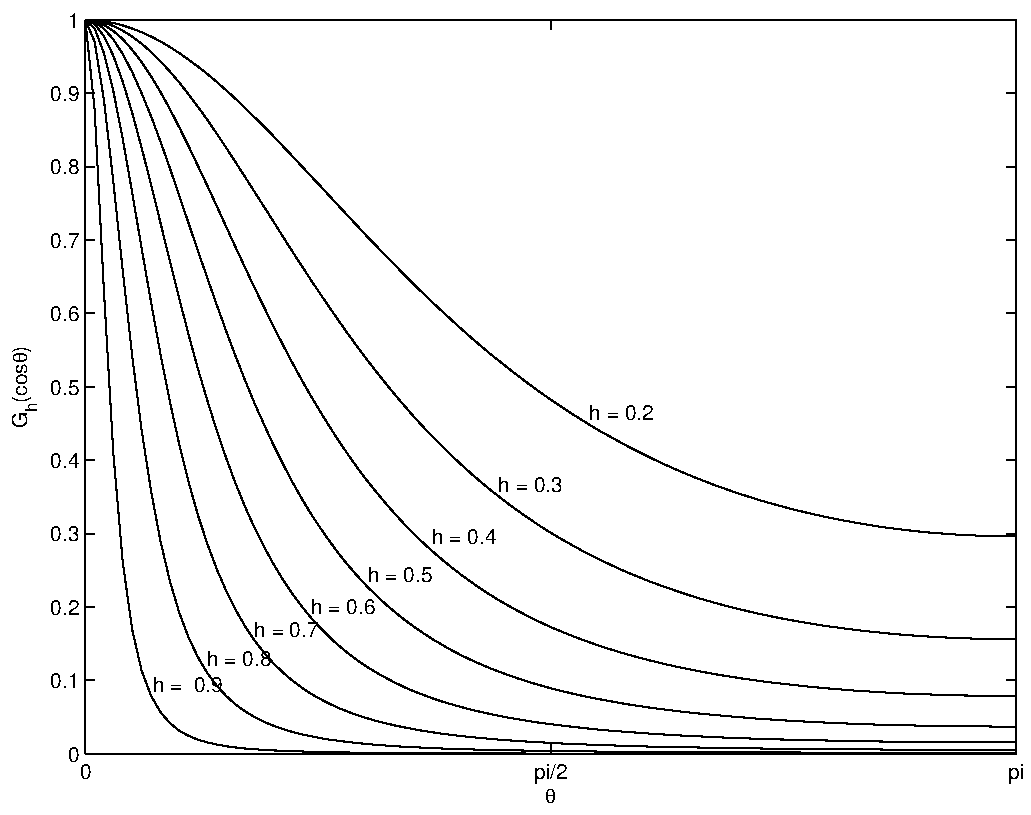
\includegraphics[width=0.45\textwidth]{images/poisson}
  }
  \hfill
  \subfigure[$h=0.8,0.9,0.955$.]
  {
    \label{Basics:Figure:SingularityKernel}
    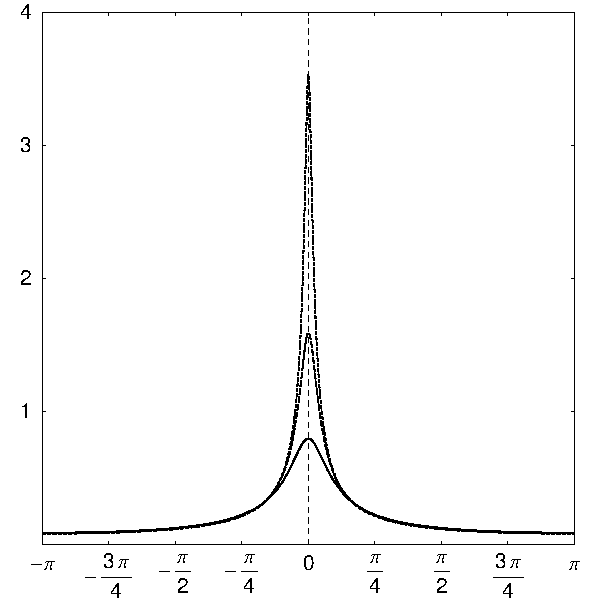
\includegraphics[width=0.45\textwidth]{images/singularity}
  }
  \caption{The kernels $\fun{Q_{h}}{\cos\vartheta}$ (left) and $\fun{S_{h}}{\cos\vartheta}$ (right)
  for different values of $h$.}
  \label{Basics:Figure:PoissonSingularityKernel}
\end{figure}

%\begin{figure}[tbp]
%  \centering
%  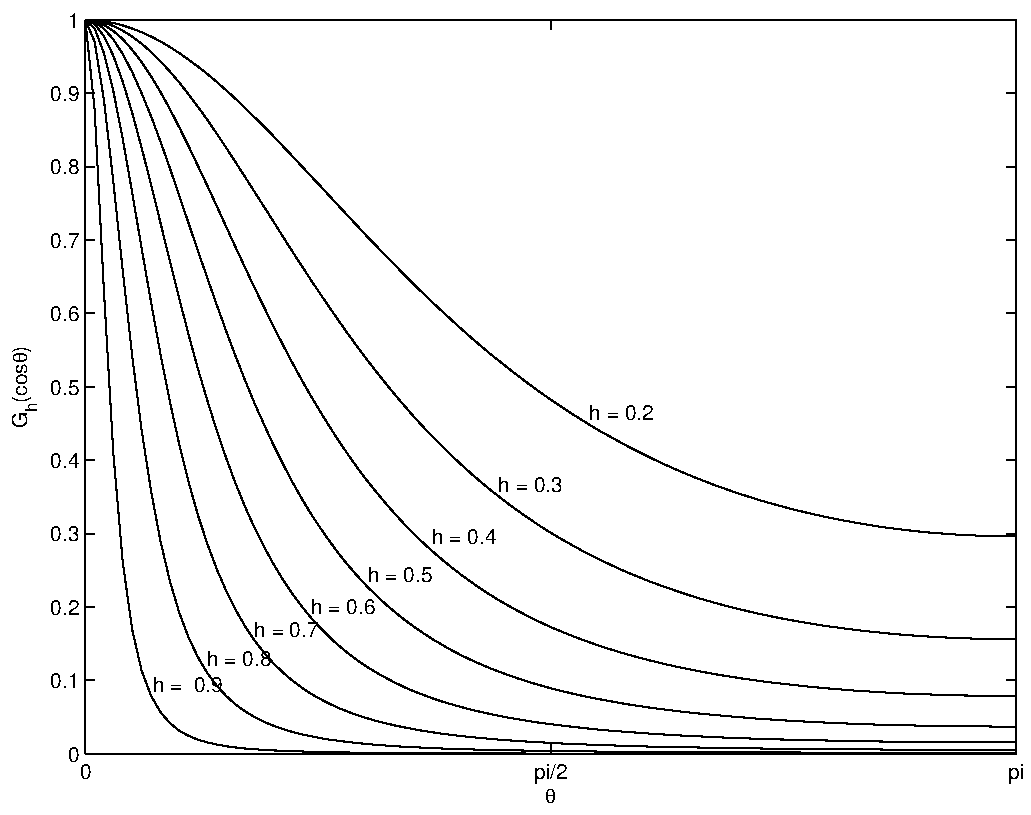
\includegraphics[width=0.9\textwidth]{images/poisson}
%  \caption{The Poisson kernel $\fun{Q_{h}}{\cos\theta}$ for $h = 0.5,0.7,0.8$ and $\theta \in \interv{[}{-\pi}{\pi}{]}$.}
%  \label{Basics:Figure:PoissonKernel}
%\end{figure}

%\begin{figure}[htb]
%  \centering
%   \subfigure[$h=0.70$]
%     {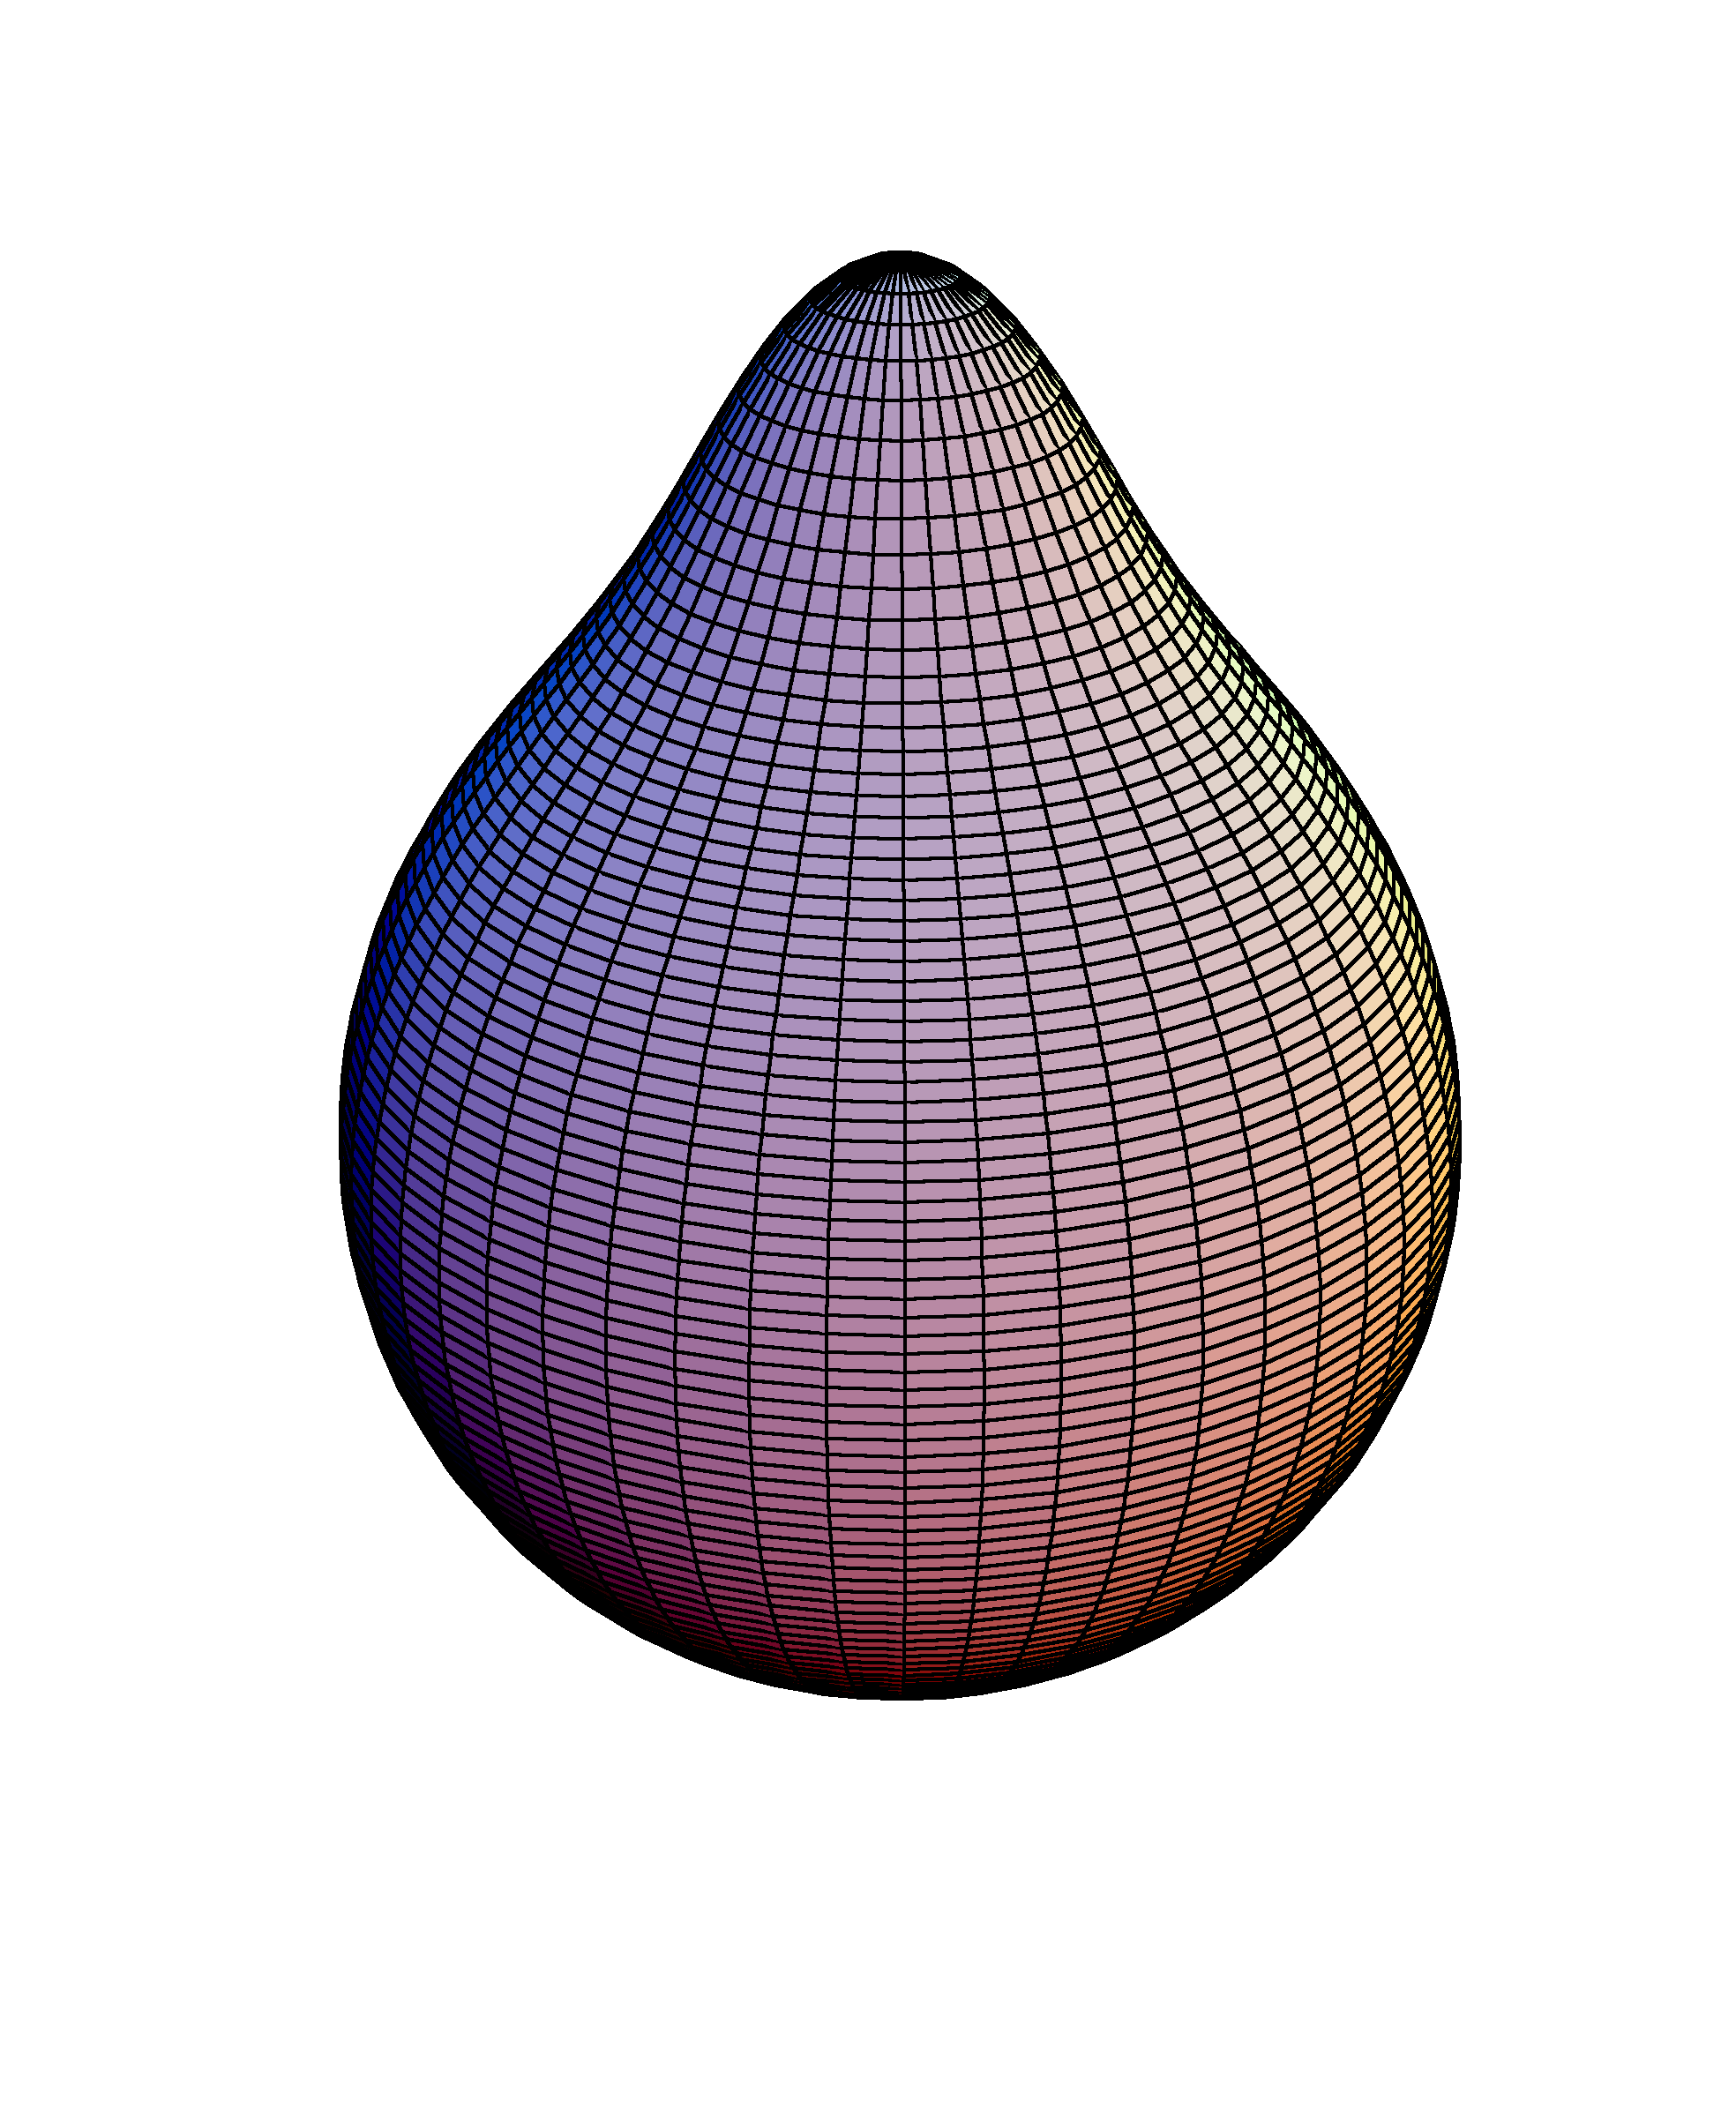
\includegraphics[width=0.5\textwidth]{images/p_070.png}}\hfill
%   \subfigure[$h=0.75$]
%     {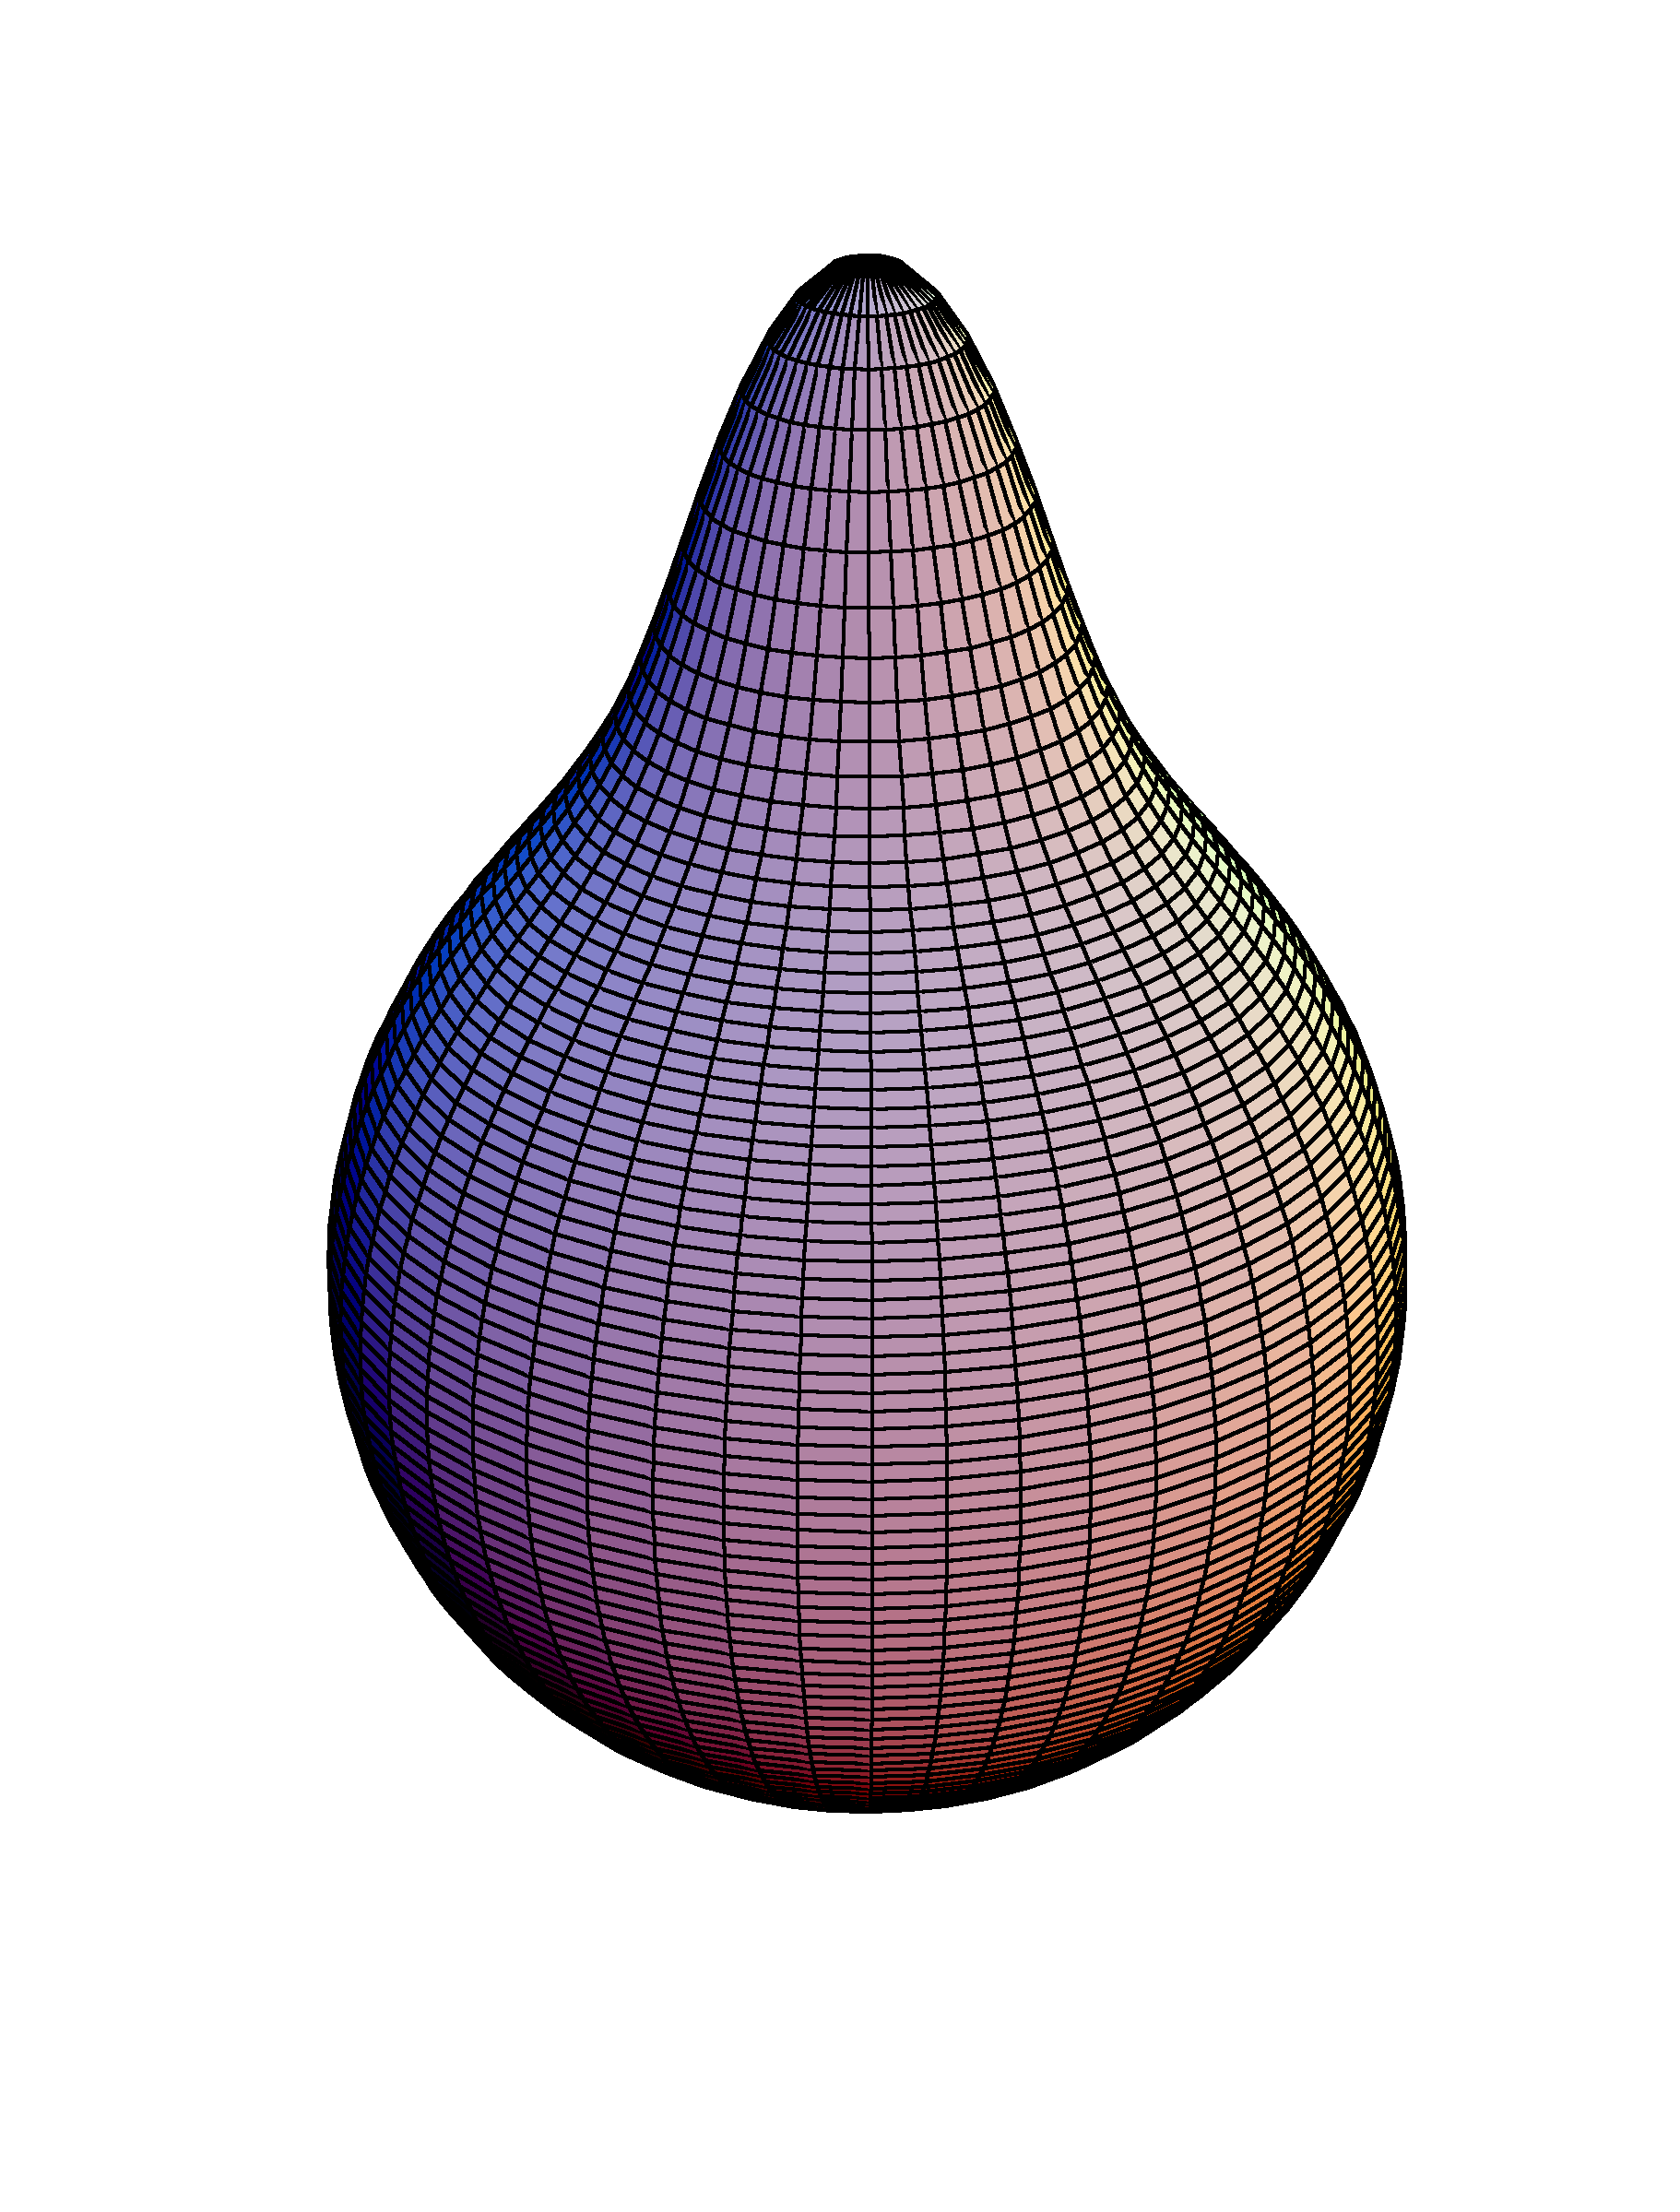
\includegraphics[width=0.5\textwidth]{images/p_075.png}}\\
%   \subfigure[$h=0.80$]
%     {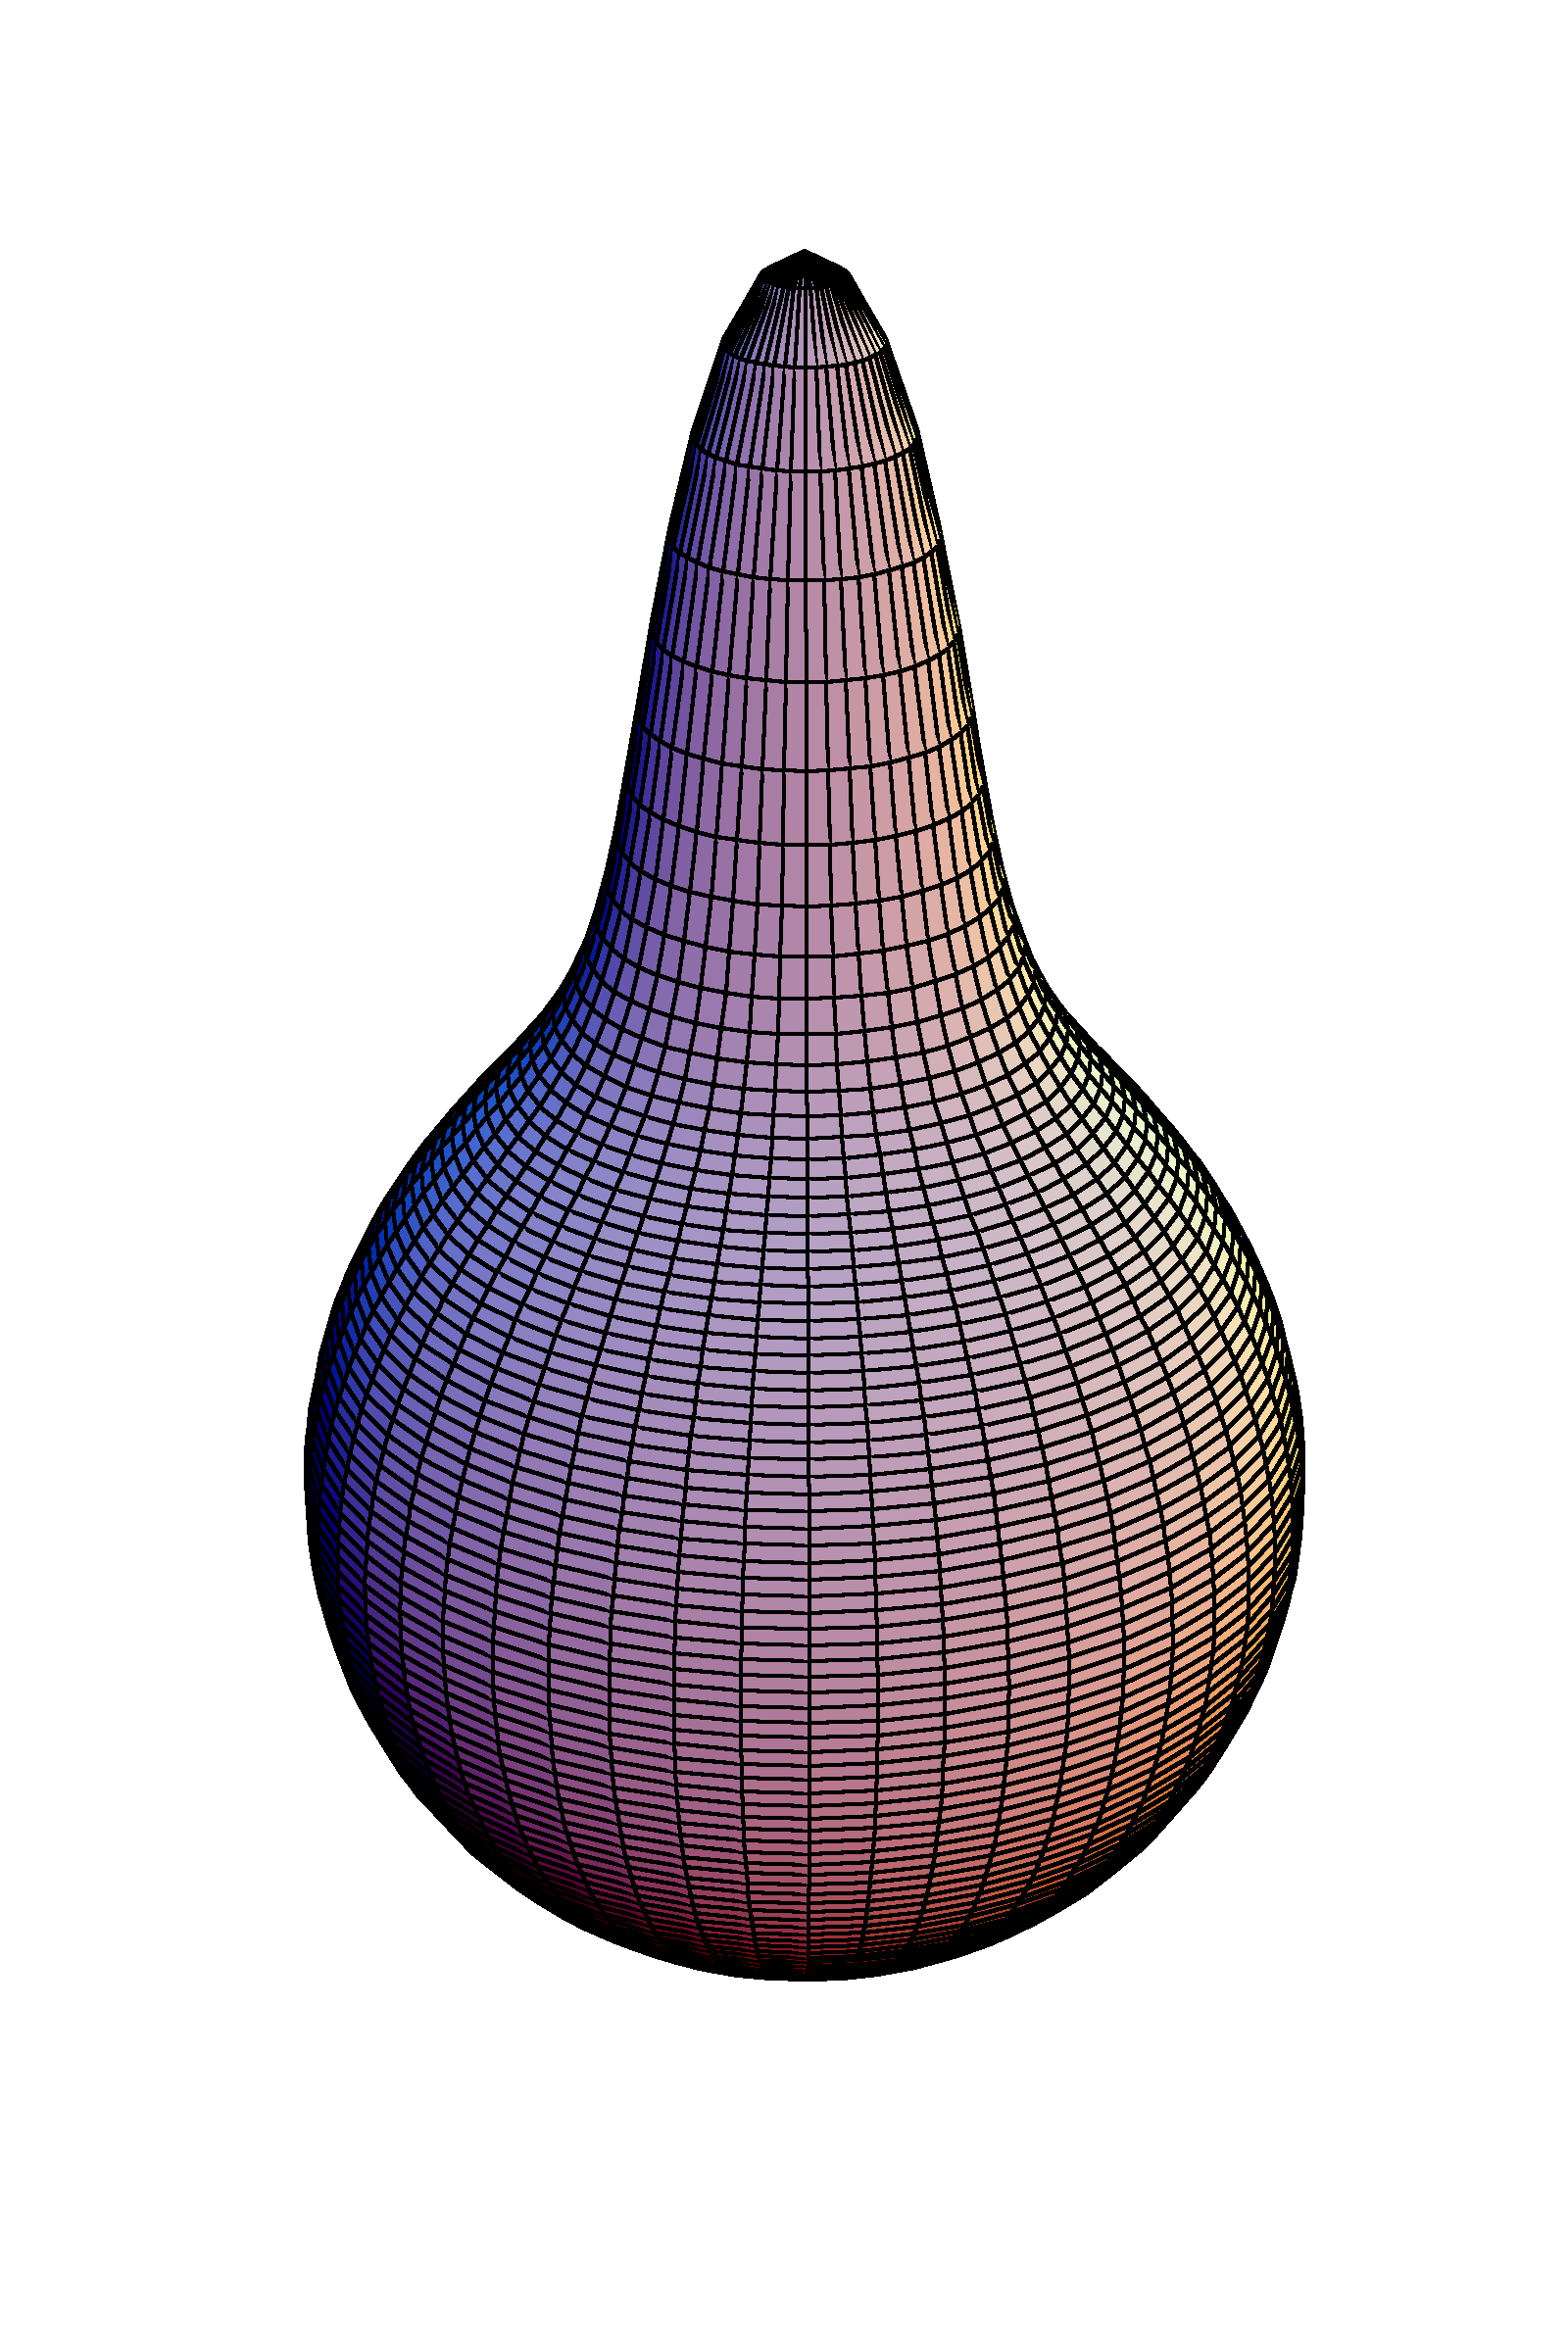
\includegraphics[width=0.5\textwidth]{images/p_080.png}}\hfill
%   \subfigure[$h=0.85$]
%     {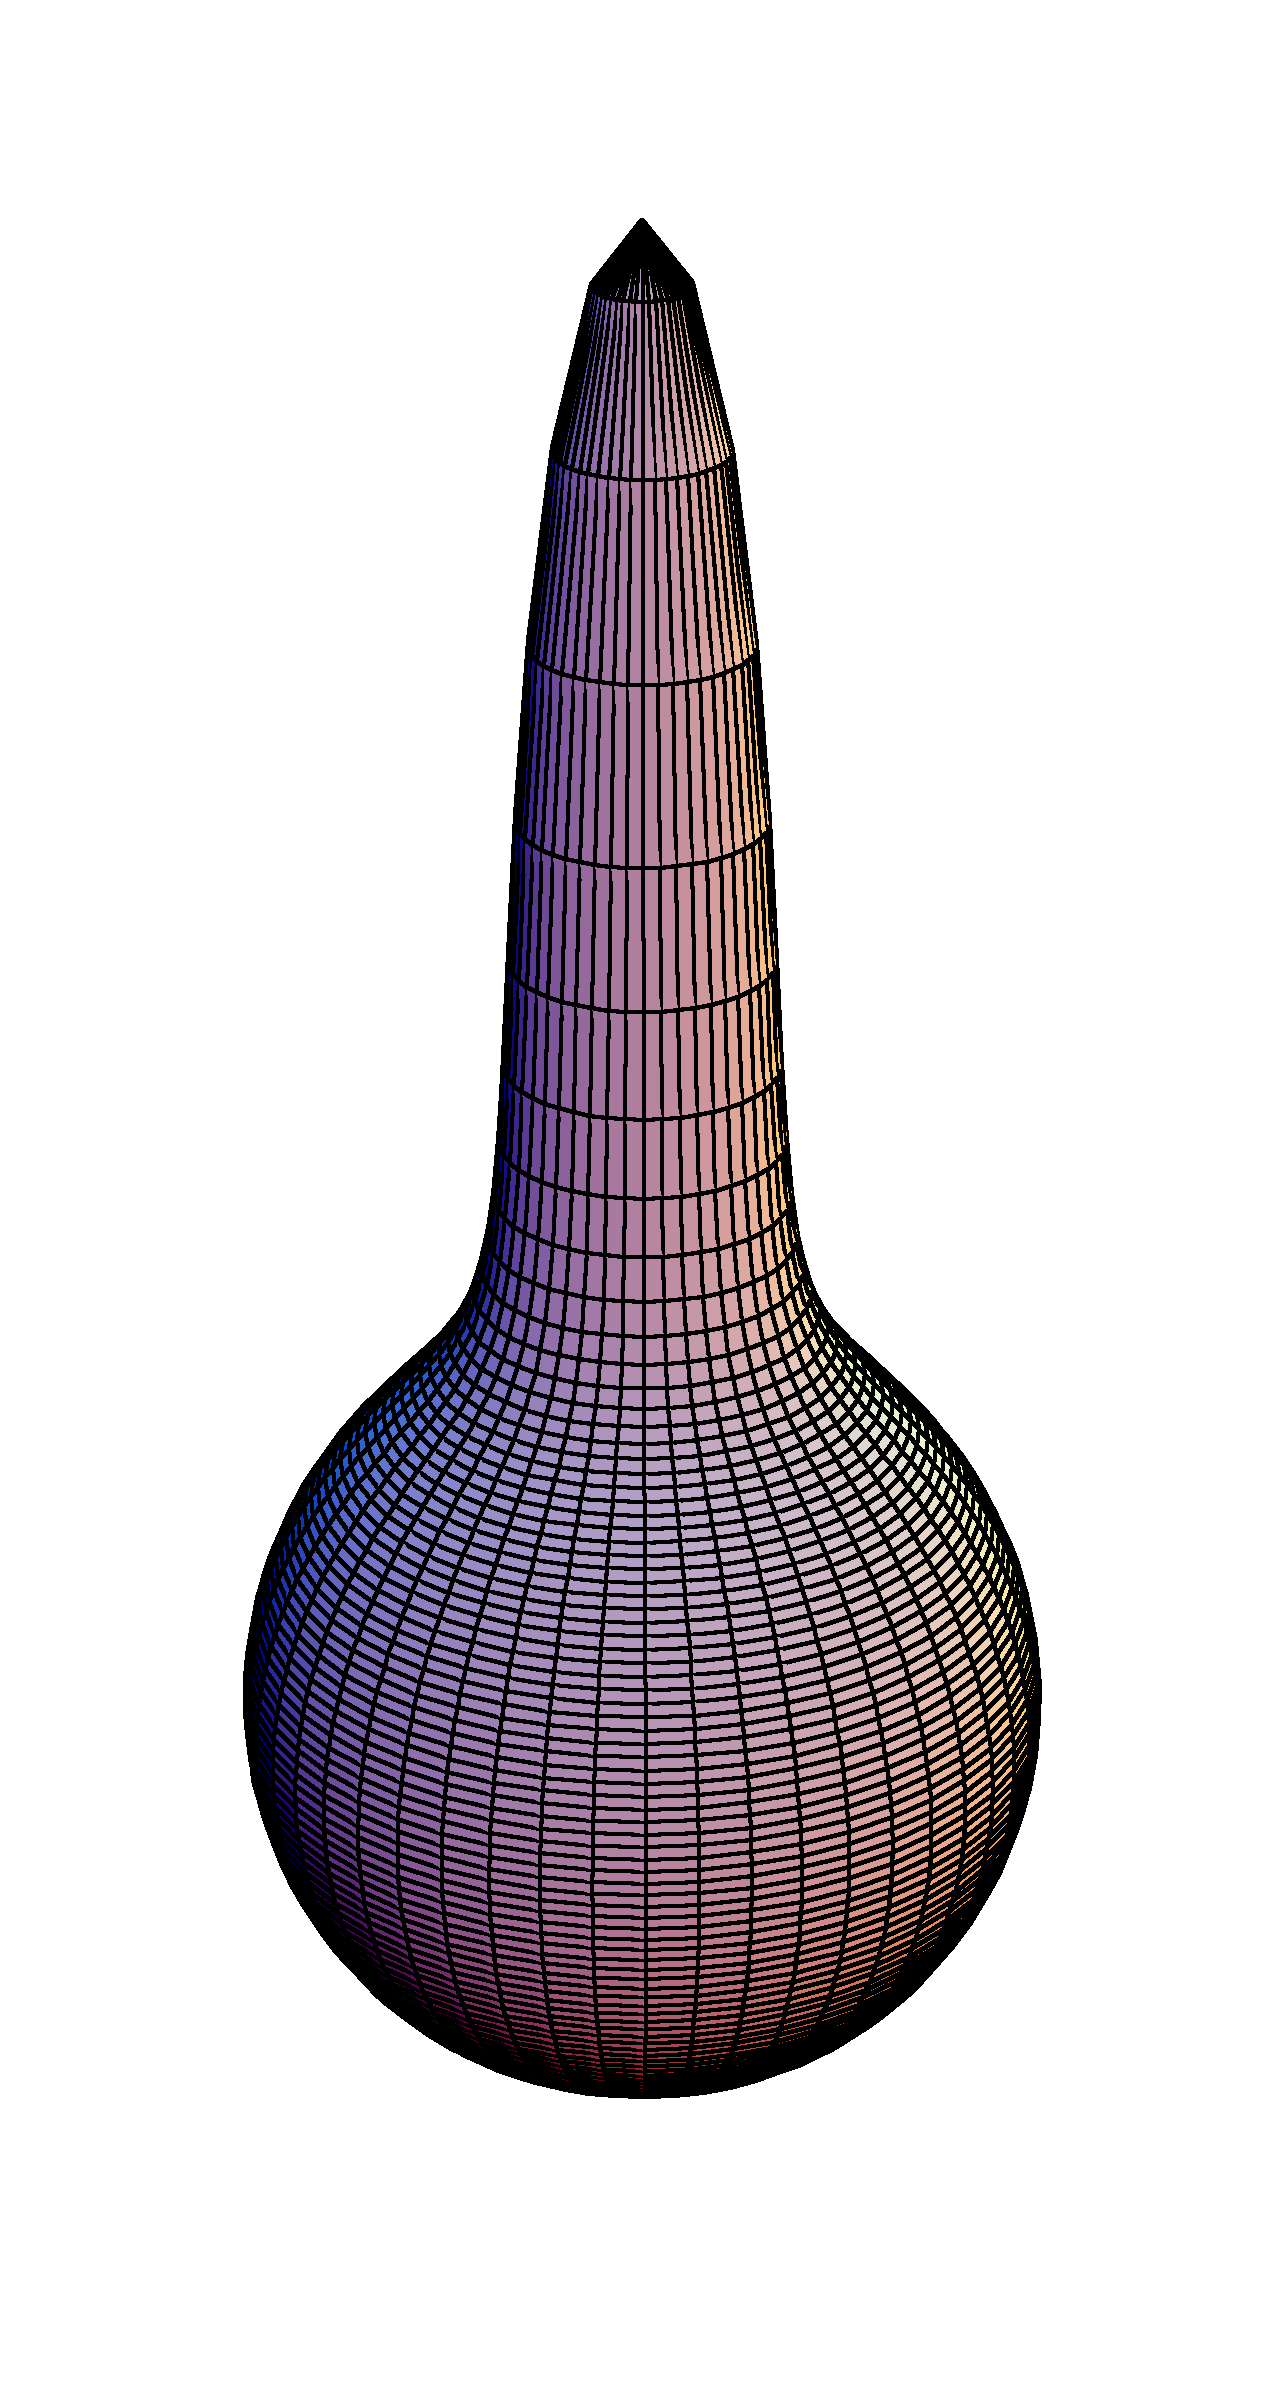
\includegraphics[width=0.5\textwidth]{images/p_085.png}}
%  \caption{The Poisson kernel plotted as a spherical radial basis function on the sphere for different values of $h$.}
%  \label{Basics:Figure:PoissonKernel2}
%\end{figure}

  The series \eqref{Basics:Solution} itself leads to a spherical radial basis function.
  \begin{definition}
    Let $h \in \interv{(}{0}{1}{)}$. The \emph{singularity kernel} 
    $S_{h}:\interv{[}{-1}{1}{]} \rightarrow \R$ is given by
    \begin{equation}
      \label{SingularityKernel}
      \fun{S_{h}}{x} := \frac{1}{2\pi} \sum_{k = 0}^{\infty} h^k \fun{P_k}{x} = 
      \frac{1}{2\pi} \frac{1}{\sqrt{1-2hx+h^2}} \quad \paren{x \in \interv{[}{-1}{1}{]}}.
    \end{equation}
  \end{definition}
  For the symbol $\fun{S_{h}^{\wedge}}{k}$, we have
  \[
    \fun{S_{h}^{\wedge}}{k} = \frac{2}{2k+1} h^k.
  \]
  See Figure \ref{Basics:Figure:SingularityKernel} and for more information \cite[pp. 112]{frgesc}.

%\begin{figure}[tbp]
%  \centering
%  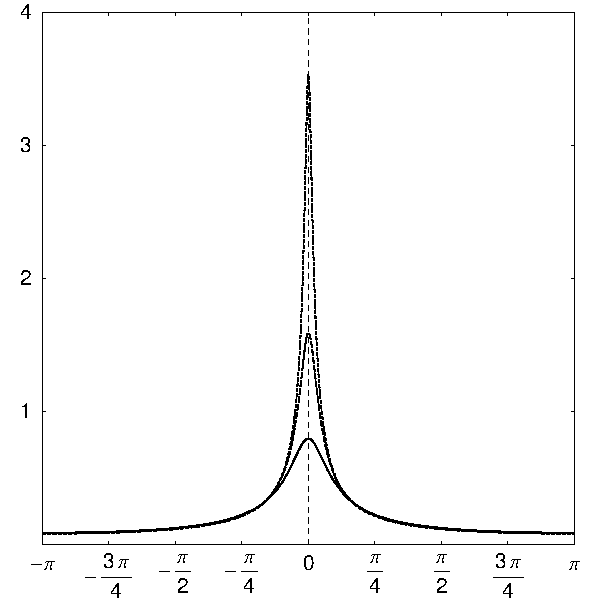
\includegraphics[width=0.7\textwidth]{images/singularity}
%  \caption{The singularity kernel $\fun{S_{h}}{\cos\theta}$ for $h = 0.8,0.9,0.955$ and $\theta \in \interv{[}{-\pi}{\pi}{]}$.}
%  \label{Basics:Figure:SingularityKernel}
%\end{figure}

%\begin{example}
%  The \emph{Gauss-Weierstra� kernel} $W_{\rho}: \interv{[}{-\pi}{\pi}{]} \rightarrow \R$ is defined by
%  \[
%    \fun{W_{\rho}}{x} := \sum_{k=0}^{\infty} \e^{-k(k+1)\rho} \frac{2k+1}{4\pi} \fun{P_{k}}{x} \quad \paren{x \in \interv{[}{-1}{1}{]}}.
%  \]
%  Results due to Bochner (\cite{bochner1950},\cite{bochner1954}) assure $\fun{W_{\rho}}{x} \ge 0$ and we have
%  \[
%    \int_{\twosphere} \fun{W_{\rho}}{\V{\eta} \cdot \V{\xi}} \dx \V{\xi} = 1.
%  \]
%  For further properties we refer to \cite{frgesc} again. The kernel function $W_{\rho}$ is illustrated in Figure \ref{Basics:Figure:GaussWeierstrassKernel}.
%\end{example}

%\begin{figure}[tb]
%  \centering
%  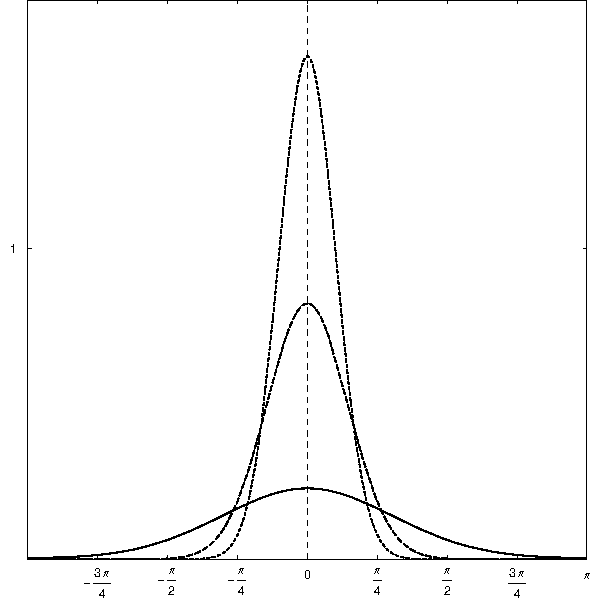
\includegraphics[width=0.7\textwidth]{images/gaussweierstrass}
%  \caption{The Gauss-Weierstra� kernel $\fun{W_{\rho}}{\cos\theta}$ for $\rho = 0.4,0.1,0.05$ and $\theta \in \interv{[}{-\pi}{\pi}{]}$.}
%  \label{Basics:Figure:GaussWeierstrassKernel}
%\end{figure}

  Locally supported zonal functions are considered for example in \cite{frsc}.
  \begin{definition}
    Let $h \in \interv{(}{0}{1}{)}$, $\lambda \in \Rp$, and $\mu \in \N$.
    \begin{enumerate}
	    \item Let the locally supported kernel
	    $L_{h,\lambda}:\interv{[}{-1}{1}{]} \rightarrow \R$ defined by
	    \[
	    \fun{L_{h,\lambda}}{x} := 
	    \left\{\begin{array}{l@{\quad \text{if} \quad}l} 
	        0 & -1 \le x \le h, \\
	        \frac{\lambda+1}{2\pi(1-h)^{\lambda+1}}\paren{x-h}^{\lambda} &  h <  x \le 1,
	      \end{array}\right.
	    \]
	    \item Furthermore, we define the iterated locally supported kernels 
	    $L_{h,\lambda}^{(\mu)}:\interv{[}{-1}{1}{]} \rightarrow \R$, $\mu \in \N$ 
	    recursively,
	    \[
	      L_{h,\lambda}^{(\mu+1)} := L_{h,\lambda}^{(\mu)} * L_{h,\lambda},
	    \]
	    where $\mu \in \N$ and $L_{h,\lambda}^{(1)} = L_{h,\lambda}$.
    \end{enumerate}
  \end{definition}  
  
	Figures \ref{Basics:Figure:LKernel} and \ref{Basics:Figure:LKernelIterated} 
	show the 
	function $L_{h,\lambda}$ for	different values $h$ and $\lambda$ and the 
	iterated kernel $L_{h,\lambda}^{(\mu)}$ for different values of $\mu$, 
	respectively.
	While the parameter $h$ again steers the localization in spatial domain, the
	parameter $\lambda$ correponds to the smoothness in spatial domain.
	The iterated kernel $L_{h,\lambda,\mu}$ trades localization in spatial domain
	for localization in frequency domain by increasing $\mu$.
	We recall the following lemma from \cite{frsc}:

	\begin{lemma}
	  \item The symbol $\fun{L_{h,\lambda}^{\wedge}}{k}$ can be computed recursively by
	    \[
	    \fun{L_{h,\lambda}^{\wedge}}{k+1} = \frac{\paren{2k+1} h}{k+\lambda+2}
	    \fun{L_{h,\lambda}^{\wedge}}{k}   - \frac{k-\lambda-1}{k+\lambda+2}
	    \fun{L_{h,\lambda}^{\wedge}}{k-1}
	    \]
	    for $k\in \N$, $\fun{L_{h,\lambda}^{\wedge}}{0} = 1$, and
	    $\fun{L_{h,\lambda}^{\wedge}}{1} = \frac{\lambda + 1 + h}{\lambda+2}$.
	\end{lemma}
	
	\begin{proof}
	  Straightforward integration yields $\fun{L_{h,\lambda}^{\wedge}}{0} = 1$
	  and $\fun{L_{h,\lambda}^{\wedge}}{1} = \frac{\lambda + 1 + h}{\lambda+2}$.
	  We use \eqref{Basics:Symbol} and apply the recurrence relation \eqref{three1}
	  and have
	  \[
	    (k+1)\fun{L_{h,\lambda}^{\wedge}}{k+1} = (2k+1)\fun{L_{h,\lambda+1}^{\wedge}}{k} +
	    (2k+1)h\fun{L_{h,\lambda}^{\wedge}}{k} -k \fun{L_{h,\lambda}^{\wedge}}{k-1}.
	  \]
	  Next, using the recurrence relation \eqref{three2} and by partial integration, we arrive at
	  \[
	    (2k+1)\fun{L_{h,\lambda+1}^{\wedge}}{k} = (\lambda+1)\paren{\fun{L_{h,\lambda}^{\wedge}}{k-1}-\fun{L_{h,\lambda}^{\wedge}}{k+1}}.
	  \]
	  The combination of these results finally yields the assertion.
	\end{proof}

\begin{figure}[tb]
  \centering
   \subfigure[$\lambda=1$]
     {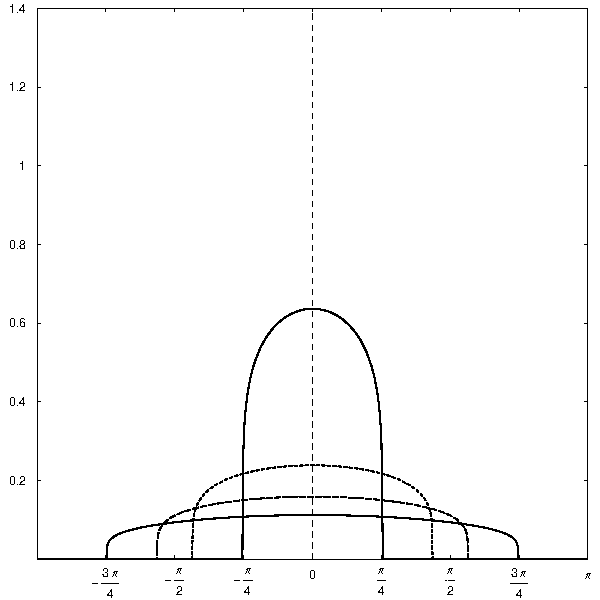
\includegraphics[width=0.45\textwidth]{images/locsup1}}\hfill
   \subfigure[$\lambda=2$]
     {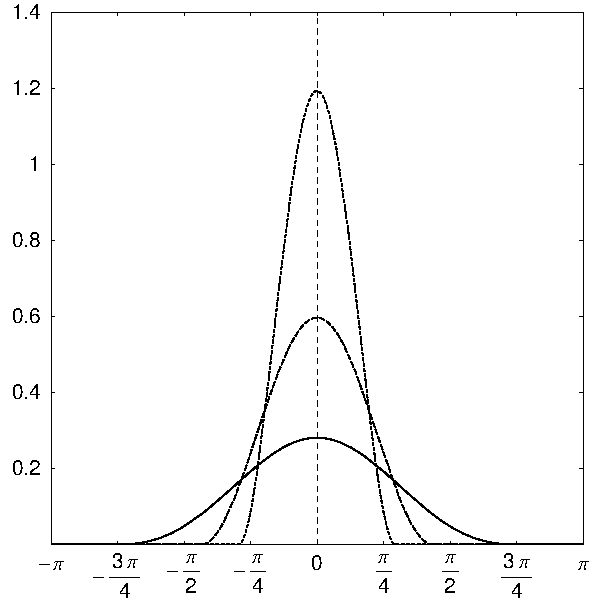
\includegraphics[width=0.45\textwidth]{images/locsup2}}
  \caption{The kernel $L_{h,\lambda}$ for $h = -0.7, 0.2, 0.6$ and different values of $\lambda$.}
  \label{Basics:Figure:LKernel}
\end{figure}

The so-called \emph{spherical Gaussian kernel} takes it's name from the bell-shaped Gaussian probability density function.

\begin{definition}
  For $\sigma>0$, the \emph{spherical Gaussian kernel}
  $G_{\sigma}:\interv{[}{-1}{1}{]} \rightarrow \R$ is given by
  \begin{equation}
    \label{GaussKernel}
    \nonumber
    \fun{G_{\sigma}}{x} := \e^{\sigma(x-1)}\,.
  \end{equation}
\end{definition}

Figure \ref{Basics:Figure:GKernel} shows the normalized function $\fun{\gamma}{\sigma}G_{\sigma}$,
$\fun{\gamma}{\sigma} := \frac{1}{\sqrt{4\pi}}\paren{\frac{1}{4\sigma}\paren{1-\e^{-4\sigma}}}^{\frac{1}{2}}$, with
$\norm{\fun{\gamma}{\sigma}G_{\sigma}}_{\Ln{2}{\twosphere}} = 1$ for different values $\sigma$.

\begin{figure}[tb]
  \centering
   \subfigure[The iterated locally supported kernel $L_{h,\lambda}^{(\mu)}$ for $h = 0.6$, $\lambda = 2$, and $\mu = 1,2,3$.]
   {
     \label{Basics:Figure:LKernelIterated}
     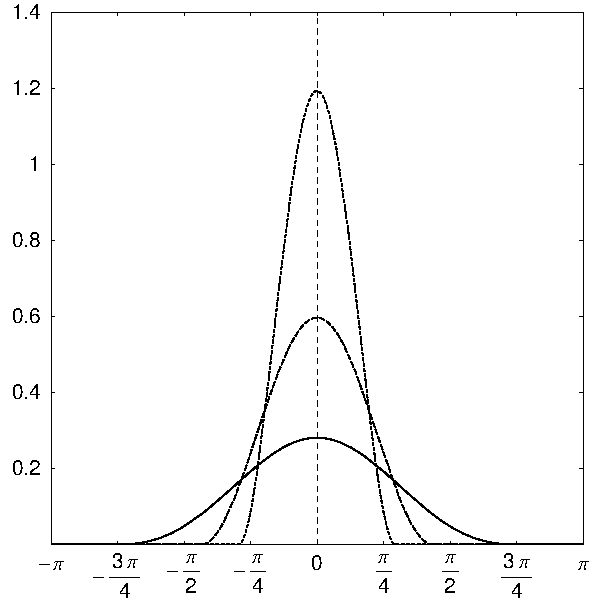
\includegraphics[width=0.45\textwidth]{images/locsup_it}
   }\hfill
   \subfigure[The Gaussian-kernel $\fun{\gamma}{\sigma}G_{\sigma}$ for $\sigma = 2,10,80$.]
   {
     \label{Basics:Figure:GKernel}
     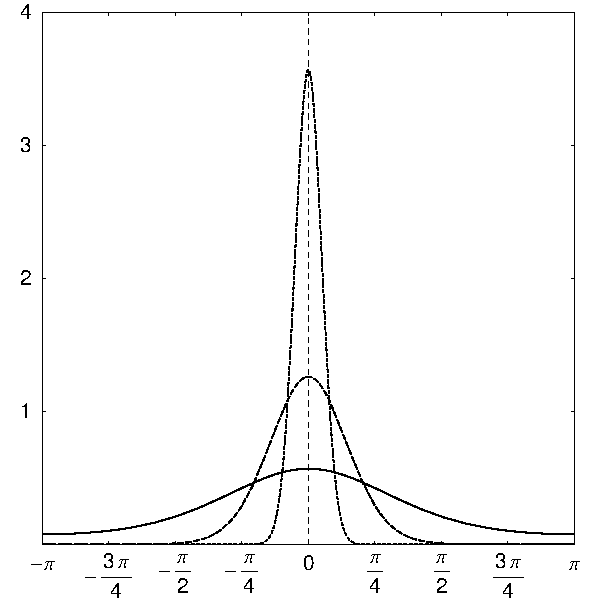
\includegraphics[width=0.45\textwidth]{images/gaussian}
   }
  \caption{}
  \label{Basics:Figure:GLKernel}
\end{figure}

As for the locally supported kernel $L_{h,\lambda}$, the Symbol $\fun{G_{\sigma}^{\wedge}}{k}$ likewise
obeys a three-term recurrence relation. A 'closed' form expression can be given in terms of Bessel functions 
of the first kind.
\begin{lemma}

  \begin{enumerate}
  \item The symbol $\fun{G_{\sigma}^{\wedge}}{k}$ can be computed by a
    recurrence relation
    \begin{equation}
      \label{Basics:Gaussian:SymbolRecurrence}
    \fun{G_{\sigma}^{\wedge}}{k+1} = 
    - \frac{2k+1}{\sigma} \fun{G_{\sigma}^{\wedge}}{k} +
    \fun{G_{\sigma}^{\wedge}}{k-1}   
    \end{equation}
    for $k\in \N$, $\fun{G_{\sigma}^{\wedge}}{0} = 4 \pi \sigma^{-1}
    \e^{-\sigma} \sinh \sigma$, and
    $\fun{G_{\sigma}^{\wedge}}{1} = \frac{2 \pi \paren{\sigma - 1 + 
    \e^{-2\sigma}\paren{1+\sigma}}}{\sigma^2}$.
  \item A 'closed' form of the symbol is given by
    \[
      \fun{G_{\sigma}^{\wedge}}{k} = \sigma^{-\frac{1}{2}} \e^{-\sigma}
      \pi^{\frac{3}{2}} \fun{I_{k+\frac{1}{2}}}{\sigma}
    \]
    where $I_{k+\frac{1}{2}}$ denotes the modified Bessel function of first kind.
    Furthermore, $\fun{G_{\sigma}^{\wedge}}{k} \ge 0$.
  \end{enumerate}
\end{lemma}
\begin{proof}
  \begin{enumerate}
  \item Integration by parts and the recurrence \eqref{three2} yield
    \begin{eqnarray*}
      (2k+1) \fun{G_{\sigma}^{\wedge}}{k} 
      & = & 2\pi \int_{-1}^1 \e^{\sigma{x-1}} (2k+1)\fun{P_{k}}{x} \; \dx x \\
      & = & 2\pi \int_{-1}^1 \e^{\sigma{x-1}} \fun{P_{k+1}'}{x} \; \dx x  - 2\pi \int_{-1}^1 \e^{\sigma{x-1}} \fun{P_{k-1}'}{x} \; \dx x \\
      & = & -\sigma 2\pi \int_{-1}^1 \e^{\sigma{x-1}} \fun{P_{k+1}}{x} \; \dx x  + \sigma 2\pi \int_{-1}^1 \e^{\sigma{x-1}} \fun{P_{k-1}}{x} \; \dx x \\
      & = & -\sigma \fun{G_{\sigma}^{\wedge}}{k+1} + \sigma \fun{G_{\sigma}^{\wedge}}{k-1}.
    \end{eqnarray*}
  \item The solution of the difference equation in \eqref{Basics:Gaussian:SymbolRecurrence} 
  is given by the modified
  Bessel function of the first kind, cf. \cite{bahu01}.
  The nonnegativity follows already from the fact that the spherical Gaussian kernel is a
  positive definite function, cf. \cite{powell}.
  \end{enumerate}
  \end{proof}
  
  \begin{remark}
    The recurrence relation \eqref{Basics:Gaussian:SymbolRecurrence} proves to be unstable. 
    This forbids computing the symbol $\fun{G_{\sigma}^{\wedge}}{k}$ in finite precision 
    arithmetic with the desired accuracy. For our numerical tests in Section 
    \ref{Applications:FastSum}, we used Mathematica 5.0 with extended precision arithmetic, 
    to compute the coefficients up to double precision accuracy. Another idea, but beyond 
    the scope of this text, would be to apply quadrature formulae to the integrals
    \[
      \fun{G_{\sigma}^{\wedge}}{k} = 2 \pi \int_{-1}^{1} \fun{G_{\sigma}}{x} \fun{P_{k}}{x} \; \dx x.
    \]
  \end{remark}

\section{Discrete Cosine Transform}
\label{Basics:DiscreteCosineTransform}

The \emph{Discrete cosine transforms (DCTs)} are a class of real transforms closely related to the 
\emph{discrete Fourier transform (DFT)}. They exploit the fact that the 
input data is real and has even symmetry. The Fourier transform of a real-even 
function is real-even and $\mathrm{i}$ times the Fourier transform of a real-odd function is real-odd. 
Similar results hold for the DFT. Based on this fact, one can now define 
real transforms respecting the additional symmetry.
Due to the discrete sampling, we have an additional choice: The symmetry can be 
viewed relatively to a data point or to a point halfway between two data points. For our 
purposes, we confine ourselves with introducing two variants.

We define the matrices
\begin{equation}
  \nonumber
  \V{C}_{N} := \paren{\cos \frac{j(2k+1) \pi}{2N}}_{j,k = 0}^{N-1}, \quad \V{D}_N := \diag\, \paren{\varepsilon_j^N}_{j = 0}^{N-1} \quad \paren{N \in \N}
\end{equation}
with $\varepsilon_0^N := \frac{1}{2}$ and $\varepsilon_j^N := 1$ for $j = 1,\ldots,N-1$.
The discrete cosine transforms DCT-II($N$) and DCT-III($N$) are then defined as follows:
\begin{equation}
  \label{Basics:DCT}
  \begin{split}
    \text{DCT-II($N$): } & \R^N \rightarrow \R^N,\ \V{\tilde{a}} := \V{C}_N\, \V{a},\\
    \text{DCT-III($N$): } & \R^N \rightarrow \R^N,\ \V{\tilde{b}} := \V{C}_N^{\transp} \V{D}_N\, \V{b}, 
  \end{split}  
\end{equation}
where $\V{a} := \paren{a_k}_{k=0}^{N-1} \in \R^N$ is the input vector and $\V{\tilde{a}} := 
\paren{\tilde{a}_j}_{j=0}^{N-1} \in \R^N$ is the output vector and similarly $\V{b}$ and $\V{\tilde{b}}$. 
The Chebyshev polynomials of the first kind $T_{k}$ are given by $\fun{T_{k}}{x} := \fun{\cos}{k \arccos x}$ 
and we obtain
\begin{equation}
  \label{Basics:DCT2}
  \begin{split}
    \tilde{a}_{j} & = \sum_{k = 0}^{N-1} a_{k} \cos \frac{j(2k+1)\pi}{2N} = \sum_{k = 0}^{N-1} a_{k} \fun{T_{j}}{\cos \frac{(2k+1) \pi}{2N}},\\
    \tilde{b}_{j} & = \sum_{k = 0}^{N-1} \varepsilon_k^N b_{k} \cos \frac{k(2j+1)\pi}{2N} = \sum_{k = 0}^{N-1} \varepsilon_k^N b_{k} \fun{T_{k}}{\cos \frac{(2j+1) \pi}{2N}},
  \end{split}  
\end{equation}
for $j = 0,\ldots,N-1$. The following lemma shows that the matrix $\V{C}_N$ is nearly, i.e. up to a scalar factor,
orthogonal (for a proof see \cite{bata}).
\begin{lemma}
  \label{Basics:DCT3}
  Let $\V{C}_N$ and $\V{D}_N$ be defined as in \eqref{Basics:DCT}. Then we have
  \[ \V{C}_N\V{C}_N^{\transp}\V{D}_N = \V{C}_N^{\transp}\V{D}_N\V{C}_N = \frac{N}{2} \V{I}_{N}. \]
\end{lemma}
Therefore the DCT-II is the inverse of the DCT-III an vice versa up to a scaling factor.

\section{Fast Polynomial Multiplication}
\label{Basics:FastPolynomialMultiplication}
A polynomial $P \in \Pol_{K}$, $K \in \N$ is uniquely determined by its \emph{Chebyshev coefficients} 
$\V{a} := \paren{a_{k}}_{k = 0}^{K}$ with $\fun{P}{x} = \sum_{k=0}^{K} a_{k} \fun{T_{k}}{x}$. Given 
now a second polynomial $Q \in \Pol_{K-1}$ with Chebyshev coefficients $\V{b} := \paren{b_{k}}_{k=0}^{K-1}$, 
we give a fast algorithm (see \cite{postta97} and \cite{kupo02}) 
for computing the Chebyshev coefficients $\V{c} := \paren{c_{k}}_{k=0}^{2K-1}$ of the polynomial 
product $R := P \cdot Q \in \Pol_{2K-1}$.\\ 
The polynomial $R$ is uniquely determined 
by the products 
\[
  f_{j} := \fun{P}{\cos \frac{(2j+1)\pi}{4K}} \fun{Q}{\cos \frac{(2j+1)\pi}{4K}}
\]
for $j = 0,\ldots,2K-1$, and by \eqref{Basics:DCT2} we obtain
\begin{eqnarray*}
  \paren{\fun{P}{\cos \frac{(2j+1)\pi}{4K}}}_{j=0}^{2K-1} = \V{C}_{2K}^{\transp} \V{a} = \V{C}_{2K}^{\transp} \paren{a_{k}}_{k=0}^{2K-1},\\
  \paren{\fun{Q}{\cos \frac{(2j+1)\pi}{4K}}}_{j=0}^{2K-1} = \V{C}_{2K}^{\transp} \V{b} = \V{C}_{2K}^{\transp} \paren{b_{k}}_{k=0}^{2K-1},
\end{eqnarray*}
where we let $a_{k} := 0$ for $k > K$ and $b_{k} := 0$ for $k > K-1$. This signifies that the evaluation 
of the polynomials $P$ and $Q$ can be performed using two DCT-IIIs of length $2K$, with an additionally 
compensation for the factors $\varepsilon_{k}^K$ introduced by the matrix $\V{D}_{2K}$ in \eqref{Basics:DCT}.
Once calculated the products $\V{f} := \paren{f_{j}}_{j=0}^{2K-1}$ with
\[
  f_{j} := \fun{P}{\cos \frac{(2j+1)\pi}{4K}} \fun{Q}{\cos \frac{(2j+1)\pi}{4K}},
\]
and taking into account that by Lemma \ref{Basics:DCT3} one verifies
$\V{C}_{2K}^{-\transp} = \frac{2}{2K} \V{D}_{2K} \V{C}_{2K}$, we finally obtain 
\[ 
  \V{c} = \frac{2}{2K} \V{D}_{2K} \V{C}_{2K} \V{f}.
\]
This leads to Algorithm \ref{Basics:Algorithm:FastPolynomialMultiplication}. The computational complexity
is $\bigo{K \log K}$ flops due to the DCT applications. Note that for our purposes, we require $K$ to be a 
power of two, although this is generally not necessary to apply the algorithm.

\begin{algorithm}[ht]
  \caption{Fast polynomial multiplication in Chebyshev representation}
  \label{Basics:Algorithm:FastPolynomialMultiplication}    
  \begin{algorithmic}
    \STATE  Input:  $K = 2^t\; (t \in \N)$, $\paren{a_{k}}_{k = 0}^{K}$, , $\paren{b_{k}}_{k = 0}^{K-1}$
    \STATE
    \STATE Evaluate the polynomials $P$ and $Q$ at the Chebyshev nodes $\paren{\cos \frac{(2j+1)\pi}{4K}}_{j = 0}^{2K-1}$
      using two fast DCT-IIIs of length $2K$.
    \STATE 
    \FOR {$j=0,\ldots , 2K-1$} 
      \STATE $f_{j} := \fun{P}{\cos \frac{(2j+1)\pi}{4K}} \fun{Q}{\cos \frac{(2j+1)\pi}{4K}}$
    \ENDFOR
    \STATE
    \STATE Compute the Chebyshev coefficients $\paren{c_{k}}_{k=0}^{2K-1}$ of $R$ using a fast DCT-II of length $2K$.
    \STATE
    \STATE Output: $\paren{c_{k}}_{k=0}^{2K-1}$
    \STATE Complexity: $\bigo{K \log K}$ flops
\end{algorithmic}
\end{algorithm}

\section{Fast Fourier Transform for Nonuniform Nodes}
\label{Basics:NFFT}

The \emph{nonuniform fast Fourier transform (NFFT)} generalizes the well known 
\emph{fast Fourier transform (FFT)}. For the sake of simplicity, we restrict 
ourselves to the one-dimensional case on the torus 
$\mathbb{T} := \pset{x \in \R}{|}{-\frac{1}{2} \le x < \frac{1}{2}}$. For 
fixed $M \in \N_{0}$ and $D \in \N$ we denote by $\mathcal{X} := \pset{x_{j} 
\in \mathbb{T}}{|}{j = 0,\ldots,D-1} \subset \mathbb{T}$ a 
\emph{sampling set} of nodes and let 
$\mathcal{I}^{M} := \pset{k \in \Z}{|}{-\frac{M}{2} 
\le k \le \frac{M}{2}-1}$ be the index set of all `admissible'
\emph{frequencies}. The considered problem is the evaluation of a 
trigonometric polynomial $f: \mathbb{T} \rightarrow \C$ with
\begin{equation}
  \label{Basics:NFFT:f}
  \fun{f}{x} := \sum_{k \in \mathcal{I}_{M}} \hat{f}_{k} \e^{- 2 \pi \im k x}
\end{equation}
on the sampling set $\mathcal{X}$. The algorithm is approximative with 
computational complexity $\bigo{M \log M + \fun{\log}{1/\varepsilon}D}$ 
where $\varepsilon$ is the desired accuracy. The technique used is to 
approximate the function $f$ in \eqref{Basics:NFFT:f} by a linear 
combination of shifted $1$-periodic window functions $\tilde{\varphi}$.
An admissible window function $\tilde{\varphi}$ should be mutually well localized 
in time and frequency.
We refer the interested reader to and \cite{postta}. Further related 
references are \cite{bey95},\cite{duro93},\cite{fesu02},\cite{four},\cite{Ja},\cite{Pe},\cite{scsc},\cite{ware98}.